\let\texyear\year % ieeeaccess.cls redefines \year, which breaks TikZ (quantikz)
\documentclass{ieeeaccess}
\usepackage{cite}
\usepackage{amsmath,amssymb,amsfonts}
\usepackage{algorithmic}
\usepackage{algorithm}
\usepackage{graphicx}
\graphicspath{{imgs/}}
\usepackage{textcomp}
\usepackage{booktabs}
\usepackage{float} % [H] placement: float stays exactly where it is in the source
\usepackage{physics}
\usepackage{multirow}
\let\accessyear\year \let\year\texyear
\usepackage{quantikz}
\let\year\accessyear
\definecolor{accessblue}{cmyk}{1,0.3,0,0.2} % class defines it as a spot color, which xcolor (loaded by TikZ) can't use
\definecolor{greycolor}{cmyk}{0,0,0,.8}
\def\xfigwd{0pt} % class captions expect \xfigwd, normally set only by its \Figure macro
\def\headerlogo{}\def\headerlogoall{} % university draft: no journal logo in the header
% university draft: footer shows only the page number, title block drops the history/DOI lines
\usepackage{etoolbox}
\makeatletter
\let\accessps@headings\ps@headings
\def\ps@headings{\accessps@headings
  \def\@oddfoot{\hfill\raisebox{8pt}{\footerpagefont\thepage}}%
  \def\@evenfoot{\raisebox{8pt}{\footerpagefont\thepage}\hfill}}
\let\accessps@titlepage\ps@titlepage
\def\ps@titlepage{\accessps@titlepage
  \def\@oddhead{}\def\@evenhead{}%
  \def\@oddfoot{\hfill\raisebox{3pt}{\footerpagefont\thepage}}%
  \def\@evenfoot{\raisebox{3pt}{\footerpagefont\thepage}\hfill}}
\pagestyle{headings}
\patchcmd{\@maketitle}{{\vss\historyfont\@history\vss}\vspace*{2mm}\par}{}{}{}
\patchcmd{\@maketitle}{{\vss\doifont Digital Object Identifier\space\@doi\vss}\vspace*{7.4mm}\par}{}{}{}
\makeatother

% ---------------------------------------------------------------
% Versión en español: separación silábica y nombres en español.
% es-minimal deja intactos los atajos (<, >, ~) que usa TikZ y la notación matemática.
\usepackage[spanish,es-minimal,es-tabla]{babel}
\addto\captionsspanish{\def\figurename{FIGURA}\def\tablename{TABLA}\def\refname{REFERENCIAS}}
\def\abstracttitle{{\color{accessblue}\abstractheadfont RESUMEN}\ifjtehm\quad\else\space\fi}
\def\indextitle{{\color{accessblue}\indexheadfont PALABRAS CLAVE}\ifjtehm\quad\else\space\fi}
\def\IEEEproofname{Demostración}
\patchcmd{\appendices}{APPENDIX}{APÉNDICE}{}{}
\floatname{algorithm}{Algoritmo}
\renewcommand{\algorithmicrequire}{\textbf{Entrada:}}
\renewcommand{\algorithmicwhile}{\textbf{mientras}}
\renewcommand{\algorithmicdo}{\textbf{hacer}}
\renewcommand{\algorithmicend}{\textbf{fin}}
\renewcommand{\algorithmicreturn}{\textbf{devolver}}
% ---------------------------------------------------------------

\newtheorem{definition}{Definición}[section]
\newtheorem{theorem}{Teorema}[section]
\newtheorem{proposition}{Proposición}[section]
\newtheorem{corollary}{Corolario}[section]
\newtheorem{lemma}{Lema}[section]

\def\BibTeX{{\rm B\kern-.05em{\sc i\kern-.025em b}\kern-.08em
    T\kern-.1667em\lower.7ex\hbox{E}\kern-.125emX}}
\begin{document}
\history{Date of publication xxxx 00, 0000, date of current version xxxx 00, 0000.}
\doi{10.1109/TQE.2020.DOI}

\title{Un estudio de la cuantificación experimental del presupuesto de privacidad en simulaciones de privacidad diferencial cuántica}
\author{\uppercase{Tomas Sierra Sanchez}\authorrefmark{1},
\uppercase{Valérie E. Gauthier-Umaña\authorrefmark{2}, y Juan F. Perez}.\authorrefmark{3}}
\address[1]{Departamento de Ingeniería de Sistemas y Computación, Universidad de los Andes (correo: t.sierras@uniandes.edu.co)}
\address[2]{Asesoría de tesis, Departamento de Ingeniería de Sistemas y Computación, Universidad de los Andes, Bogotá D.C., Colombia}
\address[3]{Asesoría de tesis, Departamento de Ingeniería Industrial, Universidad de los Andes, Bogotá D.C., Colombia (correo: jf.perez33@uniandes.edu.co)}

\markboth
{Sierra Sanchez \headeretal: Cuantificación experimental del presupuesto de privacidad en simulaciones de privacidad diferencial cuántica}
{Sierra Sanchez \headeretal: Cuantificación experimental del presupuesto de privacidad en simulaciones de privacidad diferencial cuántica}

\begin{abstract}

La privacidad diferencial es la promesa de que los datos de un solo individuo no pueden extraerse de un estudio en su conjunto. Esta investigación explora si los mecanismos de ruido cuántico pueden cumplir esta promesa. Zhou y Ying propusieron cotas teóricas para el presupuesto de privacidad de los mecanismos de ruido cuántico, así como un algoritmo para estimarlo experimentalmente. Tomando su trabajo como base, estudiamos el presupuesto de privacidad que se alcanza sobre el conjunto de datos German Credit. Proponemos una metodología de codificación para llevar los datos a simulaciones cuánticas y un flujo experimental que compara el presupuesto de privacidad experimental con las cotas teóricas de los mecanismos despolarizante, de amortiguamiento de amplitud generalizado y de amortiguamiento de fase y amplitud, tanto en el escenario central como en el local. También proponemos un experimento para entender qué garantiza realmente la publicación clásica de los datos cuánticos privatizados. En el escenario central, el presupuesto de privacidad experimental estuvo por debajo de la cota superior teórica en todos los casos, y la cota lo superó por un factor de entre 1.3 y 3.4. En el escenario local, el presupuesto experimental alcanzó la cota teórica para las variables categóricas con un número par de categorías, gracias a características tanto de la medición como de la codificación. Por último, el experimento de medición mostró que la publicación clásica de una variable categórica alcanza su presupuesto de privacidad local, y que el costo de la privacidad aparece en la desviación estándar del estimador publicado, que creció entre 1.8 y 2.8 veces después del ruido.

\end{abstract}

\begin{keywords}
Privacidad diferencial, Computación cuántica, Ruido cuántico
\end{keywords}

\titlepgskip=-15pt

\maketitle

\section{Introducción}
\label{sec:introduction}
\PARstart{A}{l} investigar o trabajar en un campo que involucra datos de otras personas, es crucial establecer límites claros sobre cómo se van a recolectar, gestionar y distribuir esos datos. Hoy en día nuestro activo más importante son los datos; por ello, se vuelve una necesidad crear herramientas que nos permitan establecer dichos límites, y una de esas herramientas es la privacidad diferencial. La privacidad diferencial describe una promesa que un custodio o curador de datos le hace al titular de los datos: ``No te verás afectado, ni negativamente ni de ninguna otra forma, por permitir que tus datos se usen en cualquier estudio o análisis, sin importar qué otros estudios, conjuntos de datos o fuentes de información estén disponibles''~\cite{dwork2014algorithmic}. En otras palabras, la privacidad diferencial es el proceso que un curador o custodio de datos debe llevar a cabo para garantizar que los datos de un solo individuo no puedan extraerse del estudio en su conjunto.

Por otro lado, la información y la computación cuánticas se están volviendo rápidamente de uso común como respuesta a la creciente necesidad de cómputo más grande y más rápido. La computación cuántica amplía significativamente las capacidades de cómputo y supera a su contraparte clásica en ciertas áreas. Dado el ruido inherente del hardware cuántico actual, se podría argumentar que es un escenario perfecto para la privacidad diferencial. De hecho, la promesa que el curador de privacidad diferencial clásica le hace al titular de los datos no cambia en el escenario cuántico; sin embargo, los medios que el curador usará para cumplir esa promesa sí cambian.

La motivación de este proyecto es entender la literatura sobre técnicas de privacidad diferencial cuántica, en particular los presupuestos de privacidad teóricos derivados por Zhou y Ying~\cite{zhou2017differential}, y contrastar esas técnicas con datos experimentales recolectados en un experimento de simulación cuántica. Con estos resultados, el proyecto espera abrir la puerta a más estudios sobre aplicaciones de la privacidad diferencial cuántica, cuyos resultados podrían seguir mejorando a medida que la computación cuántica siga creciendo.

Nuestras principales contribuciones consisten en la propuesta y el posterior estudio de una serie de experimentos que miden el presupuesto de privacidad $\epsilon$ con el que se protegen los datos, tanto en el escenario central como en el local de la privacidad diferencial, y lo comparan con el presupuesto teórico. Estos experimentos se ejecutaron como simulaciones cuánticas en el marco de Python PennyLane~\cite{bergholm2018pennylane} usando datos clásicos. Como los datos clásicos necesitan una forma de traducirse a qubits para que el simulador los use, también proponemos métodos de codificación para los distintos tipos de variables usados a lo largo de los experimentos. Por último, estudiamos qué sucede cuando los datos cuánticos con ruido se miden y se publican como un estadístico clásico, y cuánto cuesta esa publicación en privacidad y en precisión.

El resto de este artículo se organiza de la siguiente manera. La Sección~\ref{sec:background} introduce las definiciones formales de los temas usados a lo largo de esta investigación, para que el lector se familiarice con cada término y metodología que se usa más adelante. La Sección~\ref{sec:related_work} discute brevemente investigaciones previas en temas afines a esta. La Sección~\ref{sec:data_processing_and_analysis} detalla el procesamiento y el análisis realizados para seleccionar, limpiar y codificar las variables clásicas en datos cuánticos utilizables. Las Secciones~\ref{sec:finding_epsilon} y~\ref{sec:measurement_release} detallan el diseño de los experimentos, y la Sección~\ref{sec:experimental_results} analiza sus resultados. Finalmente, la Sección~\ref{sec:discussion_and_conclusion} reúne las conclusiones de la investigación en su conjunto y discute posibles trabajos futuros.

\section{Marco teórico}
\label{sec:background}

En esta sección introducimos los antecedentes que el lector puede encontrar útiles para entender la investigación. Primero presentamos los conceptos de información cuántica usados a lo largo del artículo: estados cuánticos, canales, la esfera de Bloch, la distancia de traza, la medición y los canales de ruido que luego se usan como mecanismos de privacidad. Luego presentamos la definición clásica de privacidad diferencial y, finalmente, su contraparte cuántica, junto con las herramientas de Zhou y Ying~\cite{zhou2017differential} para obtener $\epsilon$ tanto teórica como experimentalmente.

\subsection{Información y computación cuánticas}

\begin{definition}
    (Estados cuánticos~\cite{watrous_quantum_channels}). Un estado cuántico del sistema X se describe mediante una matriz de densidad $\rho$ cuyas entradas son números complejos y cuyos índices (tanto de filas como de columnas) se han puesto en correspondencia con el conjunto de estados clásicos $\Sigma$.
    \label{def:quantum_state}
\end{definition}

\begin{definition}
    (Estado mixto~\cite{zhou2017differential}). Un estado mixto de un sistema cuántico es un ensamble

    \[
      \mathbb{E} = \{(p_1,\ket{\psi_1}),...,(p_k,\ket{\psi_k})\}
    \]

    que a su vez puede representarse mediante el operador de densidad

    \[
      \rho_{\mathbb{E}} = \sum_{i}p_i\ket{\psi_i}\bra{\psi_i}
    \]

    de modo que el $\rho_{\mathbb{E}}$ resultante es la representación del ensamble como matriz de densidad.
    \label{def:mixed_state}
\end{definition}

\begin{definition}
    (Canal cuántico~\cite{watrous_quantum_channels}). Un canal cuántico describe una transformación lineal sobre matrices de densidad.
    \label{def:quantum_channel}
\end{definition}

Los canales cuánticos son importantes porque son la generalización de una operación sobre un estado cuántico, y en el caso de este proyecto necesitamos usar operaciones como el canal despolarizante, que se define gracias a esta definición general.

\begin{definition}
    (Esfera de Bloch~\cite{watrous_quantum_channels}). La esfera de Bloch es una representación geométrica útil para un solo qubit.
    \label{def:bloch_sphere}
\end{definition}

\begin{definition}
  (Representación de un estado cuántico en la esfera de Bloch~\cite{watrous_bloch_sphere}). Un estado puro de un qubit puede escribirse en términos de dos ángulos $\theta \in [0, \pi]$ y $\phi \in [0, 2\pi)$ como
  \[
    \ket{\psi} = \cos\left(\frac{\theta}{2}\right)\ket{0} + e^{i\phi}\sin\left(\frac{\theta}{2}\right)\ket{1},
  \]
  y su matriz de densidad es
  \[
    \ket{\psi}\bra{\psi} = \frac{\mathbb{I} + \sin\theta\cos\phi\, X + \sin\theta\sin\phi\, Y + \cos\theta\, Z}{2},
  \]
  que corresponde al punto $(\sin\theta\cos\phi, \sin\theta\sin\phi, \cos\theta)$ sobre la superficie de la esfera de Bloch. Los estados mixtos son combinaciones convexas de estados puros, así que corresponden a puntos dentro de la esfera: todo estado puede escribirse como
  \[
    \rho = \frac{\mathbb{I} + xX + yY + zZ}{2}, \qquad x^2 + y^2 + z^2 \leq 1,
  \]
  donde $(x, y, z)$ es su vector de Bloch. El estado completamente mixto $\mathbb{I}/2$ se ubica en el centro, $(0, 0, 0)$.
  \label{def:bloch_representation}
\end{definition}

\begin{definition}
    (Distancia de traza~\cite{zhou2017differential}). Es la distancia entre dos operadores de densidad y se define como:

    \[
      \tau(\rho, \sigma) = \frac{1}{2}Tr\abs{\rho - \sigma}
    \]

    donde $Tr(x)$ es la traza de la matriz de densidad $x$.
    \label{def:trace_distance}
\end{definition}

Otra forma útil de definir la distancia de traza en términos de vectores, según Nielsen y Chuang~\cite{Nielsen_Chuang_2010}, es

\begin{definition}
    (Distancia de traza~\cite{Nielsen_Chuang_2010}). Es la distancia entre dos vectores de qubit $u$ y $v$, definida como:

    \[
      \tau(u, v) = \frac{1}{2}\norm{u - v}
    \]
    \label{def:trace_distance_vector}
\end{definition}

\begin{definition}
    (Medición cuántica~\cite{zhou2017differential}). Es la forma de extraer información de un sistema cuántico. Matemáticamente, una medición se modela como un conjunto de matrices $M = \{K_m\}$ que cumple la condición

    \[
      \sum_m K^{\dagger}_{m}K_{m} = I
    \]

    donde $I$ es la identidad del operador de densidad (es decir, para un qubit, $I$ es la matriz identidad de $2\times2$).
    \label{def:quantum_measurement}
\end{definition}

Cuando hablemos de privacidad diferencial cuántica más adelante, no importará realmente en qué colapsa el estado cuántico. Dada esta libertad, podemos definir un POVM (\textit{Positive Operator-Valued Measure}, medida con valores en operadores positivos), que es una simplificación de la medición en la que obtenemos un conjunto de matrices $M = \{M_m\}$ con $M_m = K^{\dagger}_{m}K_{m}$ $\forall m$. Esto es posible porque solo nos interesan las probabilidades, de modo que $p_m = Tr(K_{m} \rho K^{\dagger}_{m}) = Tr(M_m\rho)$.

\begin{definition}
    (Ruido cuántico~\cite{zhou2017differential}). Es un proceso físico inherente que ocurre sobre el estado cuántico y que hace que este cambie de alguna manera.
    \label{def:quantum_noise}
\end{definition}

Para los propósitos de esta investigación nos interesan tres tipos de ruido: amortiguamiento de amplitud generalizado, amortiguamiento de fase y amplitud, y ruido despolarizante. Cada uno de estos tipos representa un proceso físico distinto, que se resume con mayor detalle en \cite{song2025hybrid} y \cite{zhou2017differential}. Las definiciones de los canales de ruido son:

\begin{definition}
    (Mecanismo de amortiguamiento de amplitud generalizado~\cite{zhou2017differential}). La operación del canal de amortiguamiento de amplitud generalizado ($\mathcal{E}_{GAD}$) sobre una matriz de densidad $\rho$ se define como

    \[
      \mathcal{E}_{GAD}(\rho) = \sum_{k = 0}^{3}E_{k}\rho E_{k}^{\dagger}
    \]

    en el espacio de Hilbert de dimensión 2

    donde

    \begin{align*}
      E_0 &= \sqrt{\eta}\begin{pmatrix} 1 & 0 \\ 0 & \sqrt{1-\gamma} \end{pmatrix}, &
      E_1 &= \sqrt{\eta}\begin{pmatrix} 0 & \sqrt{\gamma} \\ 0 & 0 \end{pmatrix}, \\
      E_2 &= \sqrt{1-\eta}\begin{pmatrix} \sqrt{1-\gamma} & 0 \\ 0 & 1 \end{pmatrix}, &
      E_3 &= \sqrt{1-\eta}\begin{pmatrix} 0 & 0 \\ \sqrt{\gamma} & 0 \end{pmatrix}
    \end{align*}

    y $\eta$ y $\gamma$ son dos parámetros,

    y el mecanismo de amortiguamiento de amplitud generalizado ($\mathcal{M}_{GAD}$) es la transformación

    \[
      \rho \mapsto \mathcal{M}_{GAD} = \mathcal{E}_{GAD}(\rho)
    \]
    \label{def:gad}
\end{definition}

\begin{definition}
    (Canal de amortiguamiento de fase~\cite{zhou2017differential}). La operación del canal de amortiguamiento de fase ($\mathcal{E}_{PD}$) sobre una matriz de densidad $\rho$ se define como

    \[
      \mathcal{E}_{PD}(\rho) = \sum_{k = 0}^{1}E_{k}\rho E_{k}^{\dagger}
    \]

    en el espacio de Hilbert de dimensión 2

    donde

    \[
      E_0 = \begin{pmatrix} 1 & 0 \\ 0 & \sqrt{1-\lambda} \end{pmatrix}, \quad
      E_1 = \begin{pmatrix} 0 & 0 \\ 0 & \sqrt{\lambda} \end{pmatrix}
    \]

    con $\lambda$ un parámetro.
    \label{def:phase_damping}
\end{definition}

\begin{definition}
    (Mecanismo de amortiguamiento de fase y amplitud~\cite{zhou2017differential}). La operación del canal de amortiguamiento de fase y amplitud ($\mathcal{E}_{PAD}$) sobre una matriz de densidad $\rho$ en el espacio de Hilbert $\mathcal{H}_2$ se define como la transformación

    \[
      \rho \mapsto \mathcal{M}_{PAD} = \mathcal{E}_{GAD}(\mathcal{E}_{PD}(\rho))
    \]
    \label{def:pad}
\end{definition}

\begin{definition}
  (Mecanismo del canal despolarizante~\cite{zhou2017differential}). La operación del canal despolarizante ($\mathcal{E}_{DEP}$) sobre una matriz de densidad $\rho$ en un espacio de Hilbert de dimensión $D$, con $I$ la matriz identidad de $D \times D$, puede representarse mediante la operación cuántica

  \[
    \mathcal{E}_{DEP}(\rho) = \frac{pI}{D} + (1-p)\rho
  \]

  donde $p$ es el parámetro de probabilidad,

  y el mecanismo despolarizante ($\mathcal{M}_{DEP}$) es la transformación

  \[
    \rho \mapsto \mathcal{M}_{DEP} = \mathcal{E}_{DEP}(\rho)
  \]
  \label{def:dep}
\end{definition}


\subsection{Privacidad diferencial}

Dwork y Roth~\cite{dwork2014algorithmic} formalizan la promesa descrita en la Sección~\ref{sec:introduction} como

\begin{definition}
    (Privacidad diferencial~\cite[Def.~2.4]{dwork2014algorithmic}). Un algoritmo aleatorizado $\mathcal{M}$ con dominio $\mathbb{N}^{|\mathcal{X}|}$ es $(\epsilon, \delta)$-diferencialmente privado si para todo $S \subseteq \mathrm{Range}(\mathcal{M})$ y para todo $x, y \in \mathbb{N}^{|\mathcal{X}|}$ tales que $\|x - y\|_1 \leq 1$:
    \[
      \Pr[\mathcal{M}(x) \in S] \leq \exp(\epsilon) \Pr[\mathcal{M}(y) \in S] + \delta,
    \]
    donde el espacio de probabilidad está dado por los lanzamientos de moneda del mecanismo $\mathcal{M}$. Si $\delta = 0$, decimos que $\mathcal{M}$ es $\epsilon$-diferencialmente privado.

    Aquí una base de datos $x \in \mathbb{N}^{|\mathcal{X}|}$ se representa por su histograma sobre el universo $\mathcal{X}$ de filas posibles ($x_i$ es el número de filas de tipo $i$), y $\|x - y\|_1 = \sum_{i} |x_i - y_i|$ es el número de registros en los que $x$ y $y$ difieren \cite[Def.~2.3]{dwork2014algorithmic}.
    \label{def:dp}
\end{definition}

En nuestra investigación nos interesa la garantía de privacidad $\epsilon$ cuando $\delta = 0$. El valor de $\epsilon$ puede interpretarse como una garantía de privacidad del algoritmo diferencialmente privado, ya que implica que agregar o quitar un registro (es decir, agregar o quitar a un participante) del conjunto de datos $x$ cambiará la probabilidad de cualquier resultado como máximo en un factor de $e^{\epsilon}$. En otras palabras, un adversario que quiera analizar el conjunto de datos no podrá distinguir de manera confiable si una persona fue incluida en él o no.

Para acotar este $\epsilon$, Dwork y Roth definen la pérdida de privacidad de un resultado como:

\begin{definition}
    (Pérdida de privacidad~\cite[Sec.~2.3]{dwork2014algorithmic}). Sean $x, y \in \mathbb{N}^{|\mathcal{X}|}$ bases de datos adyacentes ($\|x - y\|_1 \leq 1$) y sea $\xi$ un resultado de $\mathcal{M}$. La pérdida de privacidad en la que se incurre al observar $\xi$ es
    \[
      \mathcal{L}^{(\xi)}_{\mathcal{M}(x) \| \mathcal{M}(y)} = \ln\left(\frac{\Pr[\mathcal{M}(x) = \xi]}{\Pr[\mathcal{M}(y) = \xi]}\right)
    \]
    \label{def:privacy_loss}
\end{definition}

Esta pérdida de privacidad se usará a lo largo de esta investigación para medir experimentalmente $\epsilon_{exp}$ en los experimentos explicados en la Sección~\ref{sec:finding_epsilon}.

Para el propósito de nuestra investigación nos interesaron los dos escenarios que pueden considerarse al trabajar con privacidad diferencial: \textbf{central} y \textbf{local}. El escenario central (o modelo del curador, como se explica en~\cite{dwork2014algorithmic} y en la Definición~\ref{def:dp}) describe cómo un tercero de confianza recibe los datos sin protección, les aplica métodos diferencialmente privados y publica los resultados calculados a partir de ellos. Por otro lado, el escenario local describe cómo cada individuo es responsable de aplicar un método diferencialmente privado a sus propios datos y luego publicar el resultado. En otras palabras, es un caso especial de la Definición~\ref{def:dp} en el que la base de datos tiene tamaño 1~\cite[Def.~12.1]{dwork2014algorithmic}.


\subsection{Privacidad diferencial cuántica}

Como se mencionó en la Sección~\ref{sec:introduction}, la promesa de la privacidad diferencial no cambia en el escenario cuántico, pero sí los medios para cumplirla. Zhou y Ying~\cite{zhou2017differential} definen la privacidad diferencial cuántica de la siguiente manera

\begin{definition}
    (Privacidad diferencial cuántica~\cite{zhou2017differential}). Sean $d \in (0,1]$ y $\epsilon,\delta > 0$ tres constantes. Una operación cuántica $\mathcal{E}$ es $(\epsilon, \delta)$-diferencialmente privada si para todo POVM $M = \{M_m\}$, para todos los resultados $S \subseteq Out(M)$ y para todas las entradas $\rho, \sigma$ tales que $\tau(\rho, \sigma)\leq d$, se cumple que:

    \[
      Pr[\mathcal{E}(\rho)\in_{M}S] \leq e^{\epsilon} Pr[\mathcal{E}(\sigma)\in_{M}S] + \delta
    \]
    \label{def:qdp}
\end{definition}

Hay muchas formas de obtener $\epsilon$ en teoría; sin embargo, Zhou y Ying propusieron el siguiente algoritmo para obtener una cantidad llamada distancia proporcional, que ayuda a obtener $\epsilon$.

\begin{definition}
    (Distancia proporcional~\cite{zhou2017differential}). Para dos operadores de densidad $\rho$ y $\sigma$, su distancia proporcional se define como:

    \[
      PD(\rho, \sigma) = \sup_{\{M_m\}, m} \max\left(\ln\frac{q_m}{p_m}, \ln\frac{p_m}{q_m}\right)
    \]

    donde el supremo se toma sobre todos los POVM $\{M_m\}$ y todos los resultados posibles $m$,

    \[
      p_m \equiv Tr[\rho M_m], \quad q_m \equiv Tr[\sigma M_m]
    \]

    son las probabilidades de obtener el resultado $m$ cuando la medición se realiza sobre $\rho$ y $\sigma$, respectivamente, y adoptamos las convenciones $\frac{0}{0} = 1$, $\frac{1}{0} = +\infty$, $\ln 0 = -\infty$, $\ln{+\infty} = +\infty$.
    \label{def:proportional_distance}
\end{definition}

\begin{proposition}[Zhou y Ying~\cite{zhou2017differential}]
    \[
      \mathrm{PD}(\rho, \sigma) = \sup_{\ket{\psi}} \max\left(\ln\frac{\bra{\psi}\rho\ket{\psi}}{\bra{\psi}\sigma\ket{\psi}}, \ln\frac{\bra{\psi}\sigma\ket{\psi}}{\bra{\psi}\rho\ket{\psi}}\right)
    \]
    donde el supremo se toma sobre todos los estados puros.
    \label{prop:pd_pure_states}
\end{proposition}

\begin{definition}
    ($\mathrm{dPD}$~\cite{zhou2017differential}). Para dos operadores de densidad $\rho$ y $\sigma$,
    \[
      \mathrm{dPD}(\rho, \sigma) = \sup_{0 < M \leq I} \ln\frac{\Tr(M\rho)}{\Tr(M\sigma)}
    \]
    de modo que
    \begin{equation}
      \mathrm{PD}(\rho, \sigma) = \max\left(\mathrm{dPD}(\rho, \sigma), \mathrm{dPD}(\sigma, \rho)\right).
      \label{eq:pd_dpd}
    \end{equation}
    \label{def:dpd}
\end{definition}

Como el lector puede observar, dPD no es más que la pérdida de privacidad que definió~\cite{dwork2014algorithmic}, y por lo tanto, si encontramos dPD, podemos encontrar $\epsilon$. El Algoritmo~\ref{alg:dpd}~\cite{zhou2017differential} es un algoritmo de programación lineal para calcular dPD entre dos operadores de densidad $\sigma$ y $\rho$ con una precisión $\mathit{acc}$.

\begin{algorithm}[!t]
  \caption{Cálculo de $\mathrm{dPD}$ \cite{zhou2017differential}}
  \label{alg:dpd}
  \begin{algorithmic}[1]
    \REQUIRE operadores de densidad $\rho$, $\sigma$ en un espacio de Hilbert $\mathcal{H}$ de dimensión $D$; precisión deseada $\mathit{acc}$
    \STATE $r \gets 0$, $r_{prev} \gets \infty$
    \WHILE{$|r - r_{prev}| > \mathit{acc}$}
      \STATE $r_{prev} \gets r$
      \STATE $r \gets \max_i (\rho_{ii}/\sigma_{ii})$
      \STATE $A \gets \rho - r\,\sigma$
      \STATE Diagonalizar $A = P \Lambda P^{\dagger}$ ($P$ unitaria, $\Lambda$ diagonal)
      \STATE $\rho \gets P^{\dagger} \rho P$
      \STATE $\sigma \gets P^{\dagger} \sigma P$
    \ENDWHILE
    \RETURN $\ln r$
  \end{algorithmic}
\end{algorithm}

\begin{theorem}[Zhou y Ying~\cite{zhou2017differential}]
    Sea $\eta = 0.5$ en $\mathcal{E}_{GAD}$. Para todas las entradas $\rho$ y $\sigma$ con $\tau(\rho, \sigma) \leq d$, el mecanismo de amortiguamiento de amplitud generalizado $\mathcal{M}_{GAD}$ proporciona $\epsilon$-privacidad diferencial, donde
    \[
      \epsilon = \ln\left[1 + \frac{2d\sqrt{1-\gamma}}{1-\sqrt{1-\gamma}}\right]
    \]
    \label{thm:epsilon_gad}
\end{theorem}

\begin{theorem}[Zhou y Ying~\cite{zhou2017differential}]
    Sea $\eta = 0.5$ en $\mathcal{E}_{GAD}$. Si el parámetro $\gamma$ de $\mathcal{E}_{GAD}$ y $\lambda$ de $\mathcal{E}_{PD}$ cumplen $\lambda \leq \gamma$, entonces para todas las entradas $\rho$ y $\sigma$ tales que $\tau(\rho, \sigma) \leq d$, el mecanismo de amortiguamiento de fase y amplitud $\mathcal{M}_{PAD}$ proporciona $\epsilon$-privacidad diferencial, donde
    \[
      \epsilon = \ln\left[1 + \frac{2d\sqrt{1-\gamma}\sqrt{1-\lambda}}{1-\sqrt{1-\gamma}\sqrt{1-\lambda}}\right]
    \]
    \label{thm:epsilon_pad}
\end{theorem}

\begin{theorem}[Zhou y Ying~\cite{zhou2017differential}]
    Para todas las entradas $\rho$ y $\sigma$ tales que $\tau(\rho, \sigma) \leq d$, el mecanismo despolarizante $\mathcal{M}_{DEP}$ en el espacio de Hilbert de dimensión $D$ proporciona $\epsilon$-privacidad diferencial, donde
    \[
      \epsilon = \ln\left[1 + \frac{1-p}{p}\, dD\right]
    \]
    \label{thm:epsilon_dep}
\end{theorem}

\begin{corollary}[Zhou y Ying~\cite{zhou2017differential}]
    Para cada $i \in [k]$, sea $\mathcal{M}_i : \mathcal{H}_i \to \mathcal{H}'_i$ un algoritmo cuántico $\epsilon_i$-diferencialmente privado, y supongamos que son independientes. Su combinación
    \[
      \mathcal{M}_{[k]} : \bigotimes_{i=1}^{k} \mathcal{H}_i \to \bigotimes_{i=1}^{k} \mathcal{H}'_i
    \]
    se define como
    \[
      \mathcal{M}_{[k]}(\rho_1, \rho_2, \dots, \rho_k) = \bigotimes_{i=1}^{k} \mathcal{M}_i(\rho_i)
    \]
    para todos los operadores de densidad $\rho_i$ en $\mathcal{H}_i$. Entonces $\mathcal{M}_{[k]}$ es $\left(\sum_{i=1}^{k} \epsilon_i\right)$-diferencialmente privado.
    \label{cor:composition}
\end{corollary}

\begin{proposition}[Posprocesamiento, Zhou y Ying~\cite{zhou2017differential}]
    Sea $\mathcal{E}$ una operación cuántica $(\epsilon, \delta)$-diferencialmente privada. Sea $\mathcal{F}$ una operación cuántica. Entonces la composición de $\mathcal{E}$ y $\mathcal{F}$:
    \[
      \mathcal{F} \circ \mathcal{E} : \rho \mapsto \mathcal{F}(\mathcal{E}(\rho))
    \]
    también es $(\epsilon, \delta)$-diferencialmente privada.
    \label{prop:post_processing}
\end{proposition}

\section{Trabajos relacionados}
\label{sec:related_work}
Era importante entender la situación investigativa y académica actual en los campos de la información y la computación cuánticas y de la privacidad diferencial. Para ello se realizó una búsqueda en distintas bases de datos, que se analizaron para conocer el número de artículos que trataban los temas mencionados. La búsqueda encontró 61 artículos relevantes centrados en estos temas, y la distribución específica de cada uno se recopila en la Figura~\ref{fig:state_of_qdp}.

\begin{figure*}[!t]
    \centering
    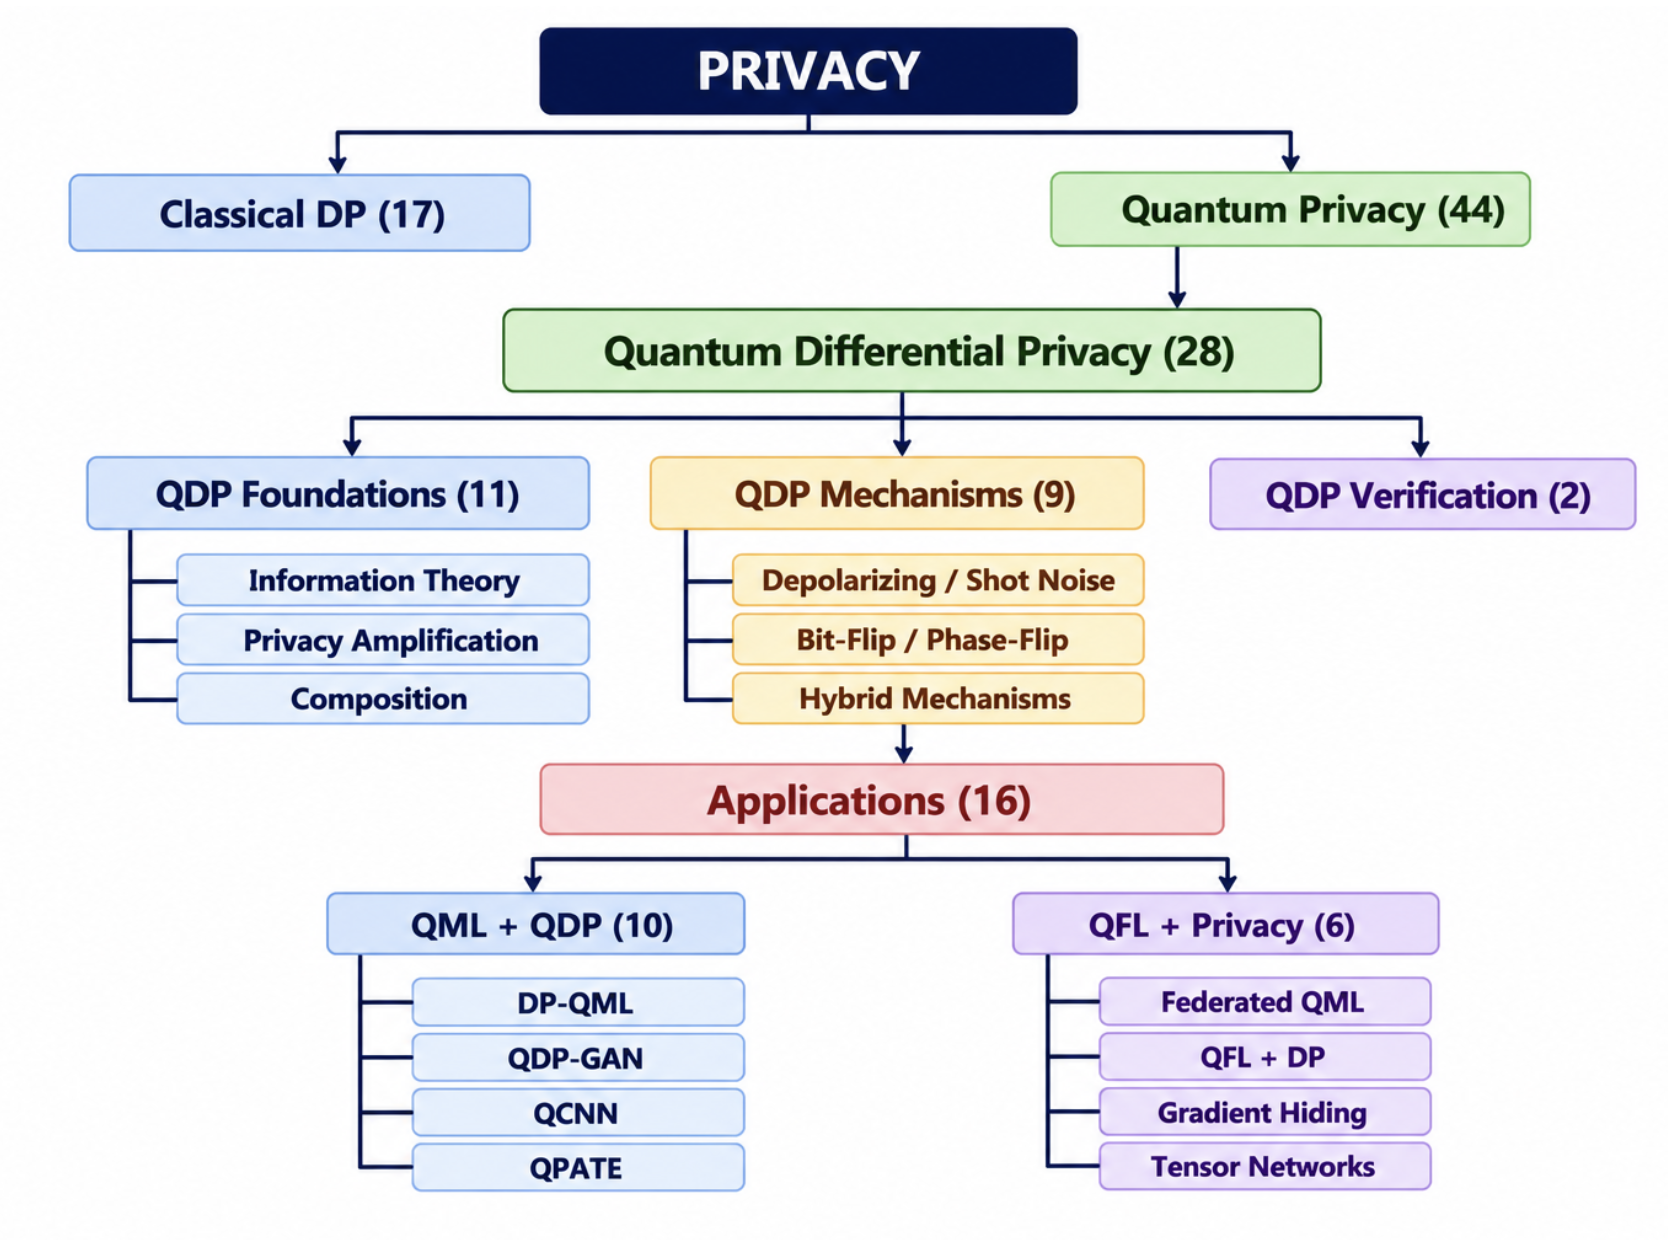
\includegraphics[width=\textwidth]{state_of_qdp.png}
    \caption{Estado del arte de la privacidad diferencial cuántica (elaboración propia, basada en la revisión de literatura descrita arriba).}
    \label{fig:state_of_qdp}
\end{figure*}

Como se muestra en la Figura~\ref{fig:state_of_qdp}, la búsqueda arrojó resultados positivos, ya que hubo muchos artículos académicos que no solo mencionaban el tema, sino que aportaban investigación valiosa y perspectivas sobre posibles enfoques que el proyecto podía tomar. Entre los más interesantes están: \cite{watkins2023quantum}, en el que se propuso un marco híbrido de aprendizaje automático cuántico que permite privacidad diferencial en el modelo; \cite{song2025hybrid}, que probó distintos mecanismos de privacidad diferencial cuántica y propuso su propia privacidad diferencial cuántica \textbf{Lifted}, que aumenta la aleatoriedad inducida en los estados cuánticos; y \cite{yang2023improved}, en el que se hizo un análisis extendido para caracterizar la protección que el ruido cuántico puede ofrecer en el contexto de algoritmos cuántico-clásicos. Por último, en el estudio de Zhou y Ying~\cite{zhou2017differential}, los autores definen un marco de privacidad diferencial en el escenario cuántico y examinan cómo distintos mecanismos de ruido cambian la protección de un presupuesto de privacidad $\epsilon$.

\section{Procesamiento y análisis de datos}
\label{sec:data_processing_and_analysis}

Esta sección detalla la metodología de procesamiento y análisis de datos que se usó para preparar el conjunto de datos clásico Statlog (German Credit Data)~\cite{hofmann1994german, germancredit2026} para su uso en el escenario cuántico. Primero describimos las características del conjunto de datos, luego los procedimientos de selección de variables y, por último, los procedimientos de codificación cuántica de los datos seleccionados.

\subsection{Descripción del conjunto de datos}

El conjunto de datos seleccionado para esta investigación es Statlog (German Credit Data), creado por el profesor Hans Hofmann \cite{hofmann1994german}. Este conjunto de datos multivariado busca clasificar a las personas como buen o mal riesgo crediticio. El conjunto original está compuesto por 1000 instancias que abarcan 21 variables (7 numéricas, 13 categóricas y la variable objetivo).

En el conjunto de datos original creado por el profesor Hofmann, todas las variables no numéricas usan un código de atributo para definir sus características (por ejemplo, el estado de una persona cuya cuenta corriente tiene menos de 0 marcos alemanes (DM) es A11). Por esa razón, se decidió que la investigación usaría una versión curada del conjunto de datos \cite{germancredit2026}, que transforma todas las etiquetas en su definición, con el fin de simplificar la comprensión del conjunto de datos por parte del lector al eliminar esa capa intermedia entre etiqueta y categoría. Toda mención del conjunto de datos en adelante se refiere a esta versión curada y no a la original compilada por el profesor Hofmann.

Un análisis de datos sencillo concluyó que el conjunto de datos no tenía ningún problema en términos de completitud (ya que todas las filas incluyen las 21 variables) ni de unicidad (ya que no hay ninguna instancia duplicada exactamente). Por estas razones, no se realizó ningún procedimiento especial de limpieza antes de la selección de variables.

\subsection{Selección de variables con PhiK}
\label{subsec:var_selection}

Para almacenar los datos cuánticos de un conjunto de datos con 1000 instancias de 20 variables cada una, la simulación tendría que guardar, como máximo, 1000 matrices de densidad de $2^n \times 2^n$, donde $n$ es el número de qubits usados. Esto significa que usar las 20 variables completas, una por qubit, implicaría $2^{20} \times 2^{20} \approx 1.1 \times 10^{12}$ entradas complejas, y a 16 bytes cada una, eso es cerca de 16 TiB por matriz. Se decidió que un estudio de correlación con respecto a la variable objetivo sería una forma adecuada de reducir esta carga. Las razones de esta decisión son: primero, la investigación no buscaba producir un clasificador y por lo tanto podía usar un número menor de variables en los experimentos. Segundo, las variables seleccionadas por un estudio de correlación serían las candidatas más probables a ser elegidas como significativas por un clasificador.

Sin embargo, como se mencionó antes, la mayoría de las variables de este conjunto de datos no son numéricas, y por lo tanto un análisis de correlación popular como la correlación de Pearson no es una opción adecuada para evaluar la correlación entre variables. Para empezar, en una variable nominal el coeficiente de Pearson depende de una elección arbitraria de etiquetas, y como las proporciones de la variable objetivo en cada categoría no son las mismas, un cambio en la etiqueta de una categoría implica un cambio en el coeficiente. Además, el coeficiente de Pearson identifica bien las relaciones lineales entre variables, pero falla en los casos no lineales.

Por estas razones se decidió usar el método PhiK \cite{BAAK2020107043PHIK} para seleccionar las variables que muestran una correlación consistentemente más fuerte con la variable objetivo. PhiK es un mejor candidato porque funciona bien tanto para variables numéricas como categóricas y es capaz de identificar relaciones no lineales entre ellas.

Usamos la librería PhiK de Baak et al. para medir la correlación y la significancia entre cada variable y la variable objetivo, y registramos los resultados en la Tabla~\ref{tab:phik}. Es importante notar que la librería devuelve dos resultados para un par de variables: el primero es $\phi_{K}$, que mide qué tan fuerte es la relación entre las dos variables. Este resultado se calcula calibrando un estadístico de prueba $\chi^2$ sobre una tabla de contingencia (poblada con las variables categóricas o con las variables numéricas agrupadas en intervalos) con respecto a una distribución normal bivariada. Esta calibración devuelve un $\phi_{K}$ con rango entre 0 (sin asociación) y 1 (asociación completa). Como $\phi_{K}$ depende de los conteos de la tabla de contingencia, renumerar las categorías ya no afecta el resultado final. El segundo resultado es $Z$, que es una conversión del valor p de la prueba de independencia a un número de desviaciones estándar. Un $Z$ más alto aporta más evidencia de que la variable no es independiente de la variable objetivo.

\begin{table}[htbp]
  \caption{Correlación $\phi_K$ de cada variable con la variable objetivo y su significancia estadística con un umbral de $Z > 2.81$.}
  \label{tab:phik}
  \centering
  \begin{tabular}{lrrc}
    \toprule
    Variable & $\phi_K$ & $Z$ & Significativa \\
    \midrule
    \texttt{status\_account}           & 0.512 & 10.965       & Sí \\
    \texttt{credit\_history}           & 0.197 & 6.912        & Sí \\
    \texttt{month\_duration}           & 0.285 & 5.648        & Sí \\
    \texttt{status\_savings}           & 0.147 & 5.283        & Sí \\
    \texttt{credit\_amount}            & 0.241 & 4.388        & Sí \\
    \texttt{collateral}                & 0.217 & 4.009        & Sí \\
    \texttt{purpose}                   & 0.204 & 3.715        & Sí \\
    \texttt{housing}                   & 0.077 & 3.601        & Sí \\
    \texttt{years\_employment}         & 0.098 & 3.053        & Sí \\
    \texttt{other\_installment\_plans} & 0.063 & 2.891        & Sí \\
    \texttt{is\_foreign\_worker}       & 0.109 & 2.545        & No  \\
    \texttt{age}                       & 0.142 & 2.177        & No  \\
    \texttt{status\_and\_sex}          & 0.123 & 1.953        & No  \\
    \texttt{secondary\_obligor}        & 0.041 & 1.835        & No  \\
    \texttt{payment\_to\_income\_ratio}& 0.075 & 1.045        & No  \\
    \texttt{telephone}                 & 0.021 & 0.689        & No  \\
    \texttt{n\_credits}                & 0.000 & 0.043        & No  \\
    \texttt{job}                       & 0.000 & $-0.390$     & No  \\
    \texttt{residence\_since}          & 0.000 & $-1.070$     & No  \\
    \texttt{n\_guarantors}             & 0.000 & $-\infty$    & No  \\
    \bottomrule
  \end{tabular}
\end{table}

Para la selección de variables elegimos usar $Z$ porque, aunque $\phi_{K}$ mide la correlación entre variables, la significancia $Z$ de esa correlación indica si es lo suficientemente significativa como para distinguirla del azar. El método de Bonferroni establece que, para asegurar que la probabilidad de al menos un falso positivo en $k$ pruebas (en nuestro caso $k = 20$, por las $20$ variables contra la variable objetivo) sea como máximo $\alpha = 0.05$, cada prueba individual debe usar un nivel de significancia de $\alpha' = \alpha/k = 0.05/20 = 0.0025$ \cite{bland1995multiple}. Aquí un falso positivo es una variable que es independiente de la variable objetivo pero que se selecciona de todos modos. Como $\alpha' = 0.0025$ corresponde a $Z \approx 2.81$, usamos $Z > 2.81$ como umbral para la selección de variables.

Como el lector puede observar en la Tabla~\ref{tab:phik}, la selección tomó 10 de las 20 variables, lo que, como se mencionó antes, deja ahora un máximo de 1000 matrices de $2^{10} \times 2^{10}$, en lugar de 1000 matrices de $2^{20} \times 2^{20}$ si usáramos un qubit por variable. En la Sección~\ref{subsec:encoding_variables} mostraremos cómo redujimos ese número. La definición y el tipo de cada variable se registran en el Apéndice~\ref{ap:selected_features}.

\subsection{Codificación de variables clásicas en estados cuánticos}
\label{subsec:encoding_variables}

Una vez elegido un conjunto reducido de variables del conjunto de datos (10 de las 20 originales), el siguiente paso fue codificar la información clásica de cada variable en qubits que pudieran usarse en la simulación cuántica. Para esto es importante notar que las variables se dividieron en dos grupos, cada uno con su propia codificación:

\subsubsection{Variables categóricas}

Son variables categóricas cuyas categorías no siguen un orden natural. Un ejemplo es la variable \texttt{purpose} (propósito), que tiene diez categorías (carro nuevo, vacaciones, educación, entre otras). Como el lector puede observar, estas categorías no siguen un orden natural, pues no hay forma de decir si, por ejemplo, carro va antes o después de educación. Por esto se decidió separarlas de las variables categóricas ordinales que se mencionarán más adelante.

La codificación propuesta para este tipo de variables está dada por la Definición~\ref{def:encoding_categorical}.

\begin{definition}
  (Método de codificación de variables categóricas). Para una variable categórica con $K$ categorías, al codificar la etiqueta $c \in \{0, \dots, K - 1\}$, el estado de qubit codificado resultante $\ket{\psi}$ está dado por la ecuación

  \[
    \ket{\psi} = RZ(\phi)H\ket{0} \quad \text{con} \quad \phi = \frac{2\pi c}{K}
  \]
  \label{def:encoding_categorical}
\end{definition}

Esta codificación deja el qubit en uno de $K$ puntos distribuidos uniformemente sobre el ecuador de la esfera de Bloch. Elegimos ubicar el qubit en el ecuador porque, a partir de la Definición~\ref{def:trace_distance_vector}, podemos expresar $\tau$ en términos del ángulo $\Delta$ entre dos puntos de un círculo y del radio de ese círculo como $r\sin{\frac{\Delta}{2}}$. Con esta expresión el lector puede notar que la distancia mínima $\tau$ se maximiza, para todos los demás ángulos sobre la esfera, cuando el radio es máximo, lo que ocurre en el ecuador de la esfera. Además, se podría argumentar que tener un $\theta$ más pequeño (es decir, el ángulo de rotación alrededor del eje y de la esfera de Bloch) reduciría $\epsilon$, y sería cierto si no fuera porque esto tiene como contrapartida hacer que las categorías sean menos distinguibles. En el caso $\theta = 0$, cualquier rotación sobre el eje z quedaría invalidada, ya que sin una rotación sobre el eje y solo agregaría una fase global.

Este método asegura entonces que $\tau$ entre dos categorías es al menos $\sin(\frac{\pi}{K})$. En teoría, esto significa que en el escenario local el $\epsilon$ final no cambiará, ya que sin importar las etiquetas que se asignen a cada categoría, el ángulo entre las etiquetas mismas puede cambiar, pero los ángulos posibles entre categorías distintas seguirán siendo los mismos. Sin embargo, lo que esta codificación no evita es que distintas categorías tengan proporciones distintas. Las etiquetas asignadas a cada categoría pueden afectar la distancia $\tau$ entre el conjunto de datos y ese mismo conjunto sin una persona, lo cual, como se explicará en la Sección~\ref{sec:finding_epsilon}, es crucial al calcular $\epsilon_{exp}$ y $\epsilon_{theo}$ y, por lo tanto, en teoría, puede llevar a resultados distintos. En el Apéndice~\ref{ap:label_categorical} recopilamos los valores de $c$ asignados a las categorías de cada variable.

\subsubsection{Variables numéricas y ordinales}

Son variables que representan rangos de una cantidad (ordinales) o que son numéricas. Un ejemplo de estas variables es \texttt{month\_duration}, que indica la duración del préstamo en meses. Un préstamo de 4 meses es claramente más corto que uno de 72, así que es importante preservar ese orden. El método de codificación que consideramos capaz de preservar este orden fue la codificación densa por ángulos (\textit{dense angle encoding})~\cite{ibm_encoding}.

Sin embargo, quedaba una pregunta: ¿qué variables se iban a codificar juntas? Para responderla, primero construimos las 15 formas posibles de agrupar las 5 variables numéricas y ordinales en dos pares y una variable sola. Luego, usamos de nuevo el método PhiK para analizar la correlación entre cada par de variables, lo cual se documenta en la Tabla~\ref{tab:phik_numerical_ordinal} (Apéndice~\ref{ap:phik_numerical_ordinal}). De este pequeño estudio se concluyó que la combinación de variables con la menor correlación en el peor caso era \texttt{status\_account} como variable sola, \texttt{status\_savings} y \texttt{month\_duration} como primer par, y \texttt{years\_employment} y \texttt{credit\_amount} como segundo par. Elegimos esta combinación porque la menor correlación en el peor par implica que cada qubit lleva la menor cantidad posible de información redundante.

Antes de la definición de la codificación, definimos una función \textbf{minmax}(min, max, a), que normaliza un valor $a \in [min , max]$ a $a \in [0 , \pi ]$.

\begin{definition}
  (Normalización min-max). Dado un valor $a \in [min , max]$ con $min, max \in \mathbb{R}$, definimos la función \textbf{minmax} como

  \[
    \textbf{minmax(min, max, a)} = \pi \times \frac{a-min}{max-min}
  \]
  \label{def:minmax}
\end{definition}

Con esta definición, el método para codificar variables numéricas y ordinales es la codificación densa por ángulos~\cite{ibm_encoding}, que definimos como:

\begin{definition}
  (Método de codificación de variables numéricas y ordinales con codificación densa por ángulos). Para una variable ordinal con $K$ categorías y una variable numérica con rango $[n_{Min}, n_{Max}]$, al codificar la variable ordinal con etiqueta $c \in \{0, \dots, K-1\}$ y la variable numérica con valor $n \in [n_{Min}, n_{Max}]$, la codificación densa por ángulos resultante está dada por

  \begin{align*}
    \ket{\psi} &= RZ(\phi)RY(\theta)\ket{0},\\
    \text{con } \phi &= minmax(n_{Min}, n_{Max}, n),\\
    \text{y } \theta &= minmax(-0.5, K - 0.5, c)
  \end{align*}
  \label{def:encoding_dense_angle}
\end{definition}

Debido a la selección de pares, la definición solo necesita cubrir el caso en el que una variable ordinal se agrupa con una numérica. Así, es importante notar que la razón por la que \textbf{minmax} se calibra de $-0.5$ a $K-0.5$ para las variables ordinales es que las categorías resultantes no puedan llegar a los polos, lo que invalidaría la compuerta RZ. Esta calibración ubica cada categoría en el centro de un intervalo de longitud $\frac{\pi}{K}$. Una excepción a esta definición es la variable sola \texttt{status\_account}, que no necesita esta calibración porque no hay compuerta RZ que invalidar, así que el rango de \textbf{minmax} es $[0, K-1]$.

Como el lector puede observar, gracias a la codificación densa por ángulos podemos reducir el número de qubits necesarios para codificar las 10 variables a 8, lo que ayuda a reducir la carga computacional de las matrices originales de $2^{10}\times 2^{10}$ (con una codificación de un qubit por variable) a matrices de $2^{8}\times 2^{8}$. El circuito cuántico final puede verse en la Figura~\ref{fig:quantum_encoding_circuit}.

\begin{figure}[!t]
  \centering
  \footnotesize
  \begin{quantikz}[row sep=0.25cm, column sep=0.3cm]
    \lstick{\texttt{collateral}~~$\ket{0}$}              & \gate{H}          & \gate{R_Z(2\pi c/K)} & \qw \\
    \lstick{\texttt{purpose}~~$\ket{0}$}                 & \gate{H}          & \gate{R_Z(2\pi c/K)} & \qw \\
    \lstick{\texttt{credit\_history}~~$\ket{0}$}         & \gate{H}          & \gate{R_Z(2\pi c/K)} & \qw \\
    \lstick{\texttt{housing}~~$\ket{0}$}                 & \gate{H}          & \gate{R_Z(2\pi c/K)} & \qw \\
    \lstick{\texttt{other\_installment\_plans}~~$\ket{0}$} & \gate{H}        & \gate{R_Z(2\pi c/K)} & \qw \\
    \lstick{\shortstack[r]{\texttt{status\_savings}\\\texttt{month\_duration}}~~$\ket{0}$}     & \gate{R_Y(\theta)} & \gate{R_Z(\phi)} & \qw \\
    \lstick{\shortstack[r]{\texttt{years\_employment}\\\texttt{credit\_amount}}~~$\ket{0}$}    & \gate{R_Y(\theta)} & \gate{R_Z(\phi)} & \qw \\
    \lstick{\texttt{status\_account}~~$\ket{0}$}         & \gate{R_Y(\theta)} & \qw                 & \qw
  \end{quantikz}
  \caption{Circuito de codificación de 8 qubits para las 10 variables seleccionadas}
  \label{fig:quantum_encoding_circuit}
\end{figure}

\section{Cálculo del presupuesto de privacidad experimental}
\label{sec:finding_epsilon}

Antes de empezar con la explicación detallada de cada experimento, es importante mencionar los parámetros de ruido elegidos para los distintos mecanismos mencionados en la Sección~\ref{sec:background}; estos se recopilan en la Tabla~\ref{tab:noise_params}. Todos estos parámetros son solo eso, parámetros, así que la selección se hizo principalmente para, primero, ejecutar todas las pruebas con los mismos parámetros y así permitir comparar los experimentos y, segundo, respetar las restricciones que imponen el Teorema~\ref{thm:epsilon_pad} sobre $\lambda$ y $\gamma$ y el Teorema~\ref{thm:epsilon_gad} sobre $\eta$. Además, por la naturaleza del mecanismo PAD, era importante elegir un $\lambda \in (0, 0.5)$ para que el mecanismo se comportara de forma distinta a GAD y DEP.

\begin{table}[H]
  \caption{Selección de parámetros para los mecanismos de ruido}
  \label{tab:noise_params}
  \centering
  \begin{tabular}{ll}
    \toprule
    Mecanismo & Parámetros\\
    \midrule
    Despolarizante & $p = 0.5$ \\
    Amortiguamiento de amplitud generalizado & $\eta = 0.5$, $\gamma = 0.5$ \\
    Amortiguamiento de fase y amplitud & $\eta = 0.5$, $\gamma = 0.5$, $\lambda = 0.25$ \\
    \bottomrule
  \end{tabular}
\end{table}

\subsection{Escenario central}
\label{subsec:experiment_central_setting}

El primer experimento que se realizó fue encontrar $\epsilon_{theo}$ y $\epsilon_{exp}$ en un escenario central para cada qubit $k$ del conjunto de datos (véase la codificación de la Sección~\ref{subsec:encoding_variables}). En otras palabras, queríamos ver qué garantía de privacidad ofrecía cada uno de los mecanismos $\mathcal{M}_{GAD}$, $\mathcal{M}_{PAD}$ y $\mathcal{M}_{DEP}$. Para lograrlo, diseñamos el flujo documentado en la Figura~\ref{fig:central_setting}.

\begin{figure*}[!t]
  \centering
  \resizebox{\textwidth}{!}{%
  \begin{tikzpicture}[
      font=\small,
      box/.style={draw, rounded corners, align=center, text width=3.3cm, minimum height=1.2cm},
      arr/.style={-latex, thick}
    ]
    % loop frames
    \draw[rounded corners] (0.3,1.5) rectangle (18.9,-7.4);
    \node[anchor=north west] at (0.45,1.45) {Para cada columna $k = 0, \dots, 7$};
    \draw[rounded corners] (0.5,-1.0) rectangle (18.7,-5.1);
    \node[anchor=south west] at (0.65,-5.05) {Para cada fila $j = 0, \dots, n-1$};
    % full dataset
    \node[box] (enc) at (2.6,0) {\textbf{Codificar}\\ $\{\rho_i^k\}_{i=0}^{n-1}$};
    \node[box] (agg) at (6.5,0) {\textbf{Agregar}\\ $\rho^k = \frac{1}{n}\sum_{i}\rho_i^k$};
    \node[box] (noise) at (10.8,0) {\textbf{Ruido}\\ $\rho^{\prime k} = \mathcal{M}(\rho^k)$};
    % neighboring dataset
    \node[box] (rem) at (2.6,-3.0) {\textbf{Quitar la fila $j$}\\ $\{\rho_i^k\}_{i \neq j}$};
    \node[box] (aggs) at (6.5,-3.0) {\textbf{Agregar}\\ $\sigma_j^k = \frac{1}{n-1}\sum_{i \neq j}\rho_i^k$};
    \node[box] (noises) at (10.8,-2.3) {\textbf{Ruido}\\ $\sigma_j^{\prime k} = \mathcal{M}(\sigma_j^k)$};
    \node[box] (dist) at (10.8,-4.1) {\textbf{Distancia de traza}\\ $d_j = \tau(\rho^k, \sigma_j^k)$};
    \node[box, text width=4.9cm] (epsj) at (15.9,-2.3) {\textbf{$\epsilon$ experimental para la fila $j$} (Alg.~\ref{alg:dpd})\\ $\epsilon_{exp}^{j} = \max\big(\mathrm{dPD}(\rho^{\prime k}, \sigma_j^{\prime k}),$\\ $\mathrm{dPD}(\sigma_j^{\prime k}, \rho^{\prime k})\big)$};
    % per-column results
    \node[box, text width=4.1cm] (theo) at (10.8,-6.5) {\textbf{$\epsilon$ teórico para la columna $k$}\\ $\epsilon_{theo}^{k} = \epsilon_{theo}(\max_j d_j)$};
    \node[box, text width=4.1cm] (expk) at (15.9,-6.5) {\textbf{$\epsilon$ experimental para la columna $k$}\\ $\epsilon_{exp}^{k} = \max_j \epsilon_{exp}^{j}$};
    % arrows
    \draw[arr] (enc) -- (agg);
    \draw[arr] (agg) -- (noise);
    \draw[arr] (enc) -- (rem);
    \draw[arr] (rem) -- (aggs);
    \draw[arr] (noise.east) -| (epsj.north);
    \draw[arr] (noises) -- (epsj);
    \draw[arr] (aggs.east) -- (8.45,-3.0) |- (noises.west);
    \draw[arr] (8.45,-3.0) |- ([yshift=-0.25cm]dist.west);
    \fill (8.65,0) circle (1.5pt);
    \draw[arr] (8.65,0) |- ([yshift=0.25cm]dist.west);
    \draw[arr] (dist) -- (theo);
    \draw[arr] (epsj) -- (expk);
  \end{tikzpicture}%
  }
  \caption{Flujo experimental para encontrar $\epsilon_{exp}$ y $\epsilon_{theo}$}
  \label{fig:central_setting}
\end{figure*}

El flujo comienza calculando algunos valores que se usarán durante el ciclo de dejar uno fuera (\textit{leave-one-out}): codificar la columna completa usando la metodología de la Sección~\ref{sec:data_processing_and_analysis}, lo que se convierte en nuestro conjunto $\{\rho_i^{k}\}$, que contiene los estados de cada persona del conjunto de datos para esa columna. Ese conjunto completo se agrega en una sola matriz $\rho^{k}$, que contiene el promedio de todos los participantes del conjunto de datos para la columna $k$. Luego se aplica a esa matriz de densidad el ruido del mecanismo seleccionado, lo que da como resultado la matriz $\rho'^{k}$. Con esas dos matrices calculadas, el flujo inicia un ciclo que recorre a cada participante del conjunto de datos para comparar el original con una versión del conjunto de datos en la que se quitó la fila $j$.

Para cada fila $j$, el proceso es el siguiente: se agrega el conjunto $\{\rho_i^{k}\}$ sin la fila $j$, lo que da como resultado la matriz de densidad $\sigma_j^{k}$, la agregación de todos los participantes excepto $j$. A partir de $\sigma_j^{k}$ se calculan tanto $\sigma_j^{\prime k}$ como $d_j$. $\sigma_j^{\prime k}$ es la matriz de densidad que resulta de aplicar el mecanismo de ruido seleccionado a $\sigma_j^{k}$, y $d_j$ es la distancia de traza entre $\rho^{k}$ y $\sigma_{j}^{k}$, que debe calcularse con las matrices antes del ruido, según los Teoremas~\ref{thm:epsilon_gad} a~\ref{thm:epsilon_dep}. Por último, se calcula $\epsilon_{exp}^{j}$, que es el $\epsilon_{exp}$ de la fila $j$ y corresponde al máximo de los valores que devuelve el Algoritmo~\ref{alg:dpd} en ambas direcciones.

Con todos esos valores, el único paso que le queda al flujo es introducirlos en cada método para encontrar $\epsilon$. Del lado teórico, el flujo introduce la distancia de traza máxima y los parámetros del mecanismo de ruido en uno de los teoremas definidos en la Sección~\ref{sec:background} (para el mecanismo despolarizante $D=2$, ya que calculamos qubit por qubit) para obtener el $\epsilon_{theo}$ de la columna. En el caso de $\epsilon_{exp}$, es el máximo $\epsilon_{exp}^{j}$ sobre todas las filas $j$, ya que esa es la máxima pérdida de privacidad que el conjunto de datos puede presentar con ese mecanismo de ruido.

Con $\epsilon_{exp}^{k}$ y $\epsilon_{theo}^{k}$ calculados para cada columna $k$ del conjunto de datos, lo único que queda es sumarlos para encontrar la cota superior de $\epsilon_{exp}$ y $\epsilon_{theo}$ del conjunto de datos. En el flujo, el curador publicaría las matrices de densidad con ruido de los 8 qubits
\[
  \bigotimes_{k=0}^{7} \rho^{\prime k} = \bigotimes_{k=0}^{7} \mathcal{M}(\rho^{k}).
\]
Por el Lema~\ref{lem:product_channel}, esto es igual a
\[
  \Big(\bigotimes_{k=0}^{7} \mathcal{M}\Big)\Big(\bigotimes_{k=0}^{7} \rho^{k}\Big) = \mathcal{M}_{[8]}(\rho^{0}, \dots, \rho^{7})
\]
que es la combinación definida en el Corolario~\ref{cor:composition}, y por lo tanto la suma es válida.

\begin{lemma}
  Para $i = 1, \dots, k$, sea $\mathcal{E}_i(\rho) = \sum_{a} E_{i,a}\, \rho\, E_{i,a}^{\dagger}$ una operación cuántica sobre $\mathcal{H}_i$ y $\rho_i$ un operador de densidad sobre $\mathcal{H}_i$. Entonces
  \[
    \Big(\bigotimes_{i=1}^{k} \mathcal{E}_i\Big)\Big(\bigotimes_{i=1}^{k} \rho_i\Big) = \bigotimes_{i=1}^{k} \mathcal{E}_i(\rho_i).
  \]
  \label{lem:product_channel}
\end{lemma}

Para facilitar la lectura, la demostración del Lema~\ref{lem:product_channel} se presenta en el Apéndice~\ref{ap:composition_proof}.

En el caso del mecanismo despolarizante, podemos modificar el flujo eliminando la necesidad de codificar cada columna por separado y aplicando el ruido a las 8 columnas completas, ya que el Teorema~\ref{thm:epsilon_dep} lo permite. Sin embargo, esto se clasifica como un experimento aparte, ya que tanto la agregación como la publicación que haría el curador se realizan sobre la matriz completa de 8 qubits (no qubit por qubit, como se explicó), por lo que no permite compararlo con el flujo original. Más adelante, en la Sección~\ref{sec:discussion_and_conclusion}, discutiremos cómo estos métodos producen resultados de privacidad muy distintos.


\subsection{Escenario local}
\label{subsec:experiment_local_setting}

Hasta ahora hemos considerado un experimento en el que un curador de confianza aplica el ruido a los datos y los publica. Este experimento, en cambio, intenta responder qué pasaría si fuera cada persona la que aplicara el ruido: el escenario local.

En el escenario central definimos como vecinas dos matrices de densidad agregadas: la de las 1000 filas completas $\rho$ y la que deja una fuera, $\sigma$. En este escenario (inspirado en~\cite[Def.~12.1]{dwork2014algorithmic}, como se mencionó en la Sección~\ref{sec:background}), sin embargo, como es una sola persona a la vez la que privatiza sus datos, no tendría sentido comparar a dos personas distintas como vecinas, ya que en realidad lo que el atacante querría saber es ``¿cuál era la categoría original de la persona A?''. Con esta idea, este experimento define como vecinos los posibles estados en los que se codifica cada etiqueta, y gracias a la Definición~\ref{def:qdp} podemos comparar dos estados como vecinos mediante su distancia de traza $\tau$. Sin embargo, este experimento limita las variables que podemos codificar. Como se mencionó en la Sección~\ref{subsec:encoding_variables}, las variables numéricas deben normalizarse dentro de la esfera de Bloch con los valores mínimo y máximo de las variables. En el escenario local una sola persona no tiene forma de acceder a esos datos y por lo tanto no puede codificarlos de esa manera. Con esa limitación en mente, este escenario calcula el $\epsilon$ de todas las variables categóricas y de la variable sola \texttt{status\_account}, ya que las otras dos variables ordinales comparten qubit con una variable numérica y por lo tanto no pueden codificarse de forma independiente. La Figura~\ref{fig:local_setting} muestra el flujo del experimento en el escenario local.
\begin{figure*}[!t]
  \centering
  \resizebox{\textwidth}{!}{%
  \begin{tikzpicture}[
      font=\small,
      box/.style={draw, rounded corners, align=center, text width=5.6cm, minimum height=1.2cm},
      arr/.style={-latex, thick}
    ]
    % pair-loop frame (same width as the central-setting figure, so both figures share one scale)
    \draw[rounded corners] (0.3,-1.0) rectangle (18.9,-4.2);
    \node[anchor=south west] at (0.45,-4.15) {Para cada par $\{c, c'\}$, $c < c'$};
    % all values of the variable
    \node[box] (enc) at (6.0,0) {\textbf{Codificar los $K$ valores} (Sec.~\ref{subsec:encoding_variables})\\[3pt] $\{\rho_c\}_{c=0}^{K-1}$};
    \node[box] (noise) at (13.2,0) {\textbf{Ruido}\\ $\rho^{\prime}_c = \mathcal{M}(\rho_c)$};
    % pair of values
    \node[box] (dist) at (6.0,-2.6) {\textbf{Distancia de traza}\\ $d_{cc'} = \tau(\rho_c, \rho_{c'})$};
    \node[box] (epsp) at (13.2,-2.6) {\textbf{$\epsilon$ experimental para el par $\{c, c'\}$} (Alg.~\ref{alg:dpd})\\[2pt] $\epsilon_{exp}^{cc'} = \max\big(\mathrm{dPD}(\rho^{\prime}_c, \rho^{\prime}_{c'}),$\\ $\mathrm{dPD}(\rho^{\prime}_{c'}, \rho^{\prime}_c)\big)$};
    % results for the variable
    \node[box] (theo) at (6.0,-5.4) {\textbf{$\epsilon$ teórico de la variable}\\ $\epsilon_{theo}(\max_{c,c'} d_{cc'})$};
    \node[box] (expk) at (13.2,-5.4) {\textbf{$\epsilon$ experimental de la variable}\\ $\max_{c,c'} \epsilon_{exp}^{cc'}$};
    % arrows
    \draw[arr] (enc) -- (noise);
    \draw[arr] (enc) -- (dist);
    \draw[arr] (noise) -- (epsp);
    \draw[arr] (dist) -- (theo);
    \draw[arr] (epsp) -- (expk);
  \end{tikzpicture}%
  }
  \caption{Flujo del experimento en el escenario local para encontrar $\epsilon$ de una variable categórica u ordinal}
  \label{fig:local_setting}
\end{figure*}

El experimento comienza definiendo dos conjuntos: $\{\rho_c\}$, que son todas las matrices de densidad que resultan de codificar la $c$-ésima etiqueta, y $\{\rho_c^{\prime}\}$, que es el conjunto de todas las matrices de densidad $\rho_c$ después de pasar por el mecanismo de ruido $\mathcal{M}$. Luego, para cada par de etiquetas $\{c, c^{\prime}\}, c < c^{\prime}$, calculamos tanto la distancia de traza entre las matrices de densidad originales sin ruido $\rho_c$ y $\rho_{c^{\prime}}$ como el $\epsilon_{exp}$, que sigue el mismo procedimiento del escenario central pero con entradas $\rho_c^{\prime}$ y $\rho_{c^{\prime}}^{\prime}$. Al final, hacemos la misma búsqueda del máximo $\epsilon_{theo}$ y $\epsilon_{exp}$ sobre todos los pares analizados, y ese es el resultado final de la variable.

\section{Medición y publicación clásica de una variable categórica}
\label{sec:measurement_release}

Con los dos experimentos anteriores pudimos encontrar $\epsilon_{theo}$ y $\epsilon_{exp}$ para ambos escenarios de la privacidad diferencial. Sin embargo, esto deja una pregunta importante por responder: ¿cómo se ve realmente este presupuesto de privacidad después de la publicación clásica de los datos? Los experimentos anteriores no necesitaban responder esta pregunta para calcular $\epsilon$, ya que teníamos la distribución completa (la matriz de densidad) de los qubits.

Para responder esta pregunta, primero debemos aclarar el concepto de \textbf{copia}. Para los propósitos de esta investigación, una copia es un qubit en un estado cuántico específico, ya sea un estado puro $\ket{\psi}$ o un estado mixto con matriz de densidad $\rho$. Cuando esa copia se mide, colapsa en uno de los dos estados de la base de medición (es decir, $\ket{+}$ o $\ket{-}$ en la base $X$). Debido al teorema de no clonación~\cite{watrous_limitations}, el curador (o cualquier persona) no puede guardar el estado antes de la medición para medirlo de nuevo, y por lo tanto cada nueva medición requiere preparar el estado completamente otra vez.

La Figura~\ref{fig:release_designs} muestra qué pasa con los datos después de los flujos de las Subsecciones~\ref{subsec:experiment_central_setting} y~\ref{subsec:experiment_local_setting}. En el escenario central, el estado final es la agregación del conjunto de datos completo, $\rho = \frac{1}{n}\sum_{i=1}^{n}\rho_i$, así que, por la ley de probabilidad total, medir una copia de $\rho^{\prime}$ no es distinto de escoger una persona $i$ al azar y luego medir su estado. En otras palabras, cada persona queda escondida dentro de la agregación completa, y la privacidad de cada copia es el $\epsilon$ calculado en la Subsección~\ref{subsec:experiment_central_setting}. Sin embargo, cada nueva copia necesaria para estimar la distribución es otra extracción y por lo tanto cuesta otro $\epsilon$, lo que da un total de $N\epsilon$ por el Corolario~\ref{cor:composition}, donde $N$ es el número de copias medidas. En el escenario local, por otro lado, cada individuo solo necesita una medición. Como una medición (Definición~\ref{def:quantum_measurement}) puede verse como una operación cuántica en sí misma, la Proposición~\ref{prop:post_processing} implica que el $\epsilon$ final es como máximo el encontrado en el experimento del escenario local.

\begin{figure*}[!t]
  \centering
  \resizebox{\textwidth}{!}{%
  \begin{tikzpicture}[
      font=\small,
      box/.style={draw, rounded corners, align=center, text width=2.8cm, minimum height=1.1cm, fill=white},
      noisebox/.style={box, fill=gray!20},
      group/.style={draw, rounded corners, thick},
      mech/.style={draw, rounded corners, dashed},
      lbl/.style={font=\footnotesize\itshape, anchor=north east},
      arr/.style={-latex, thick}
    ]
    % ---------- C: central setting (Sec. V-A) ----------
    \node[anchor=west] at (0.3,2.0) {\textbf{C: escenario central}};
    \draw[group] (0.3,-1.1) rectangle (2.7,1.5);
    \node[anchor=north west] at (0.4,1.45) {Individuo};
    \node[box, text width=1.2cm] (ci) at (1.5,-0.2) {$\rho_i$};
    \draw[group] (3.4,-1.1) rectangle (18.9,1.5);
    \node[anchor=north west] at (3.5,1.45) {Curador};
    \draw[mech] (3.7,-0.95) rectangle (14.1,0.95);
    \node[lbl] at (14.05,0.93) {mecanismo central de QDP (Sec.~\ref{subsec:experiment_central_setting})};
    \node[box] (call) at (5.4,-0.25) {$\rho_0, \dots, \rho_{n-1}$};
    \node[box] (cagg) at (8.9,-0.25) {\textbf{Agregar}\\ $\rho = \frac{1}{n}\sum_i \rho_i$};
    \node[noisebox] (cnoise) at (12.4,-0.25) {\textbf{Ruido}\\ $\rho^{\prime} = \mathcal{M}(\rho)$};
    \node[box] (cmeas) at (16.4,-0.25) {\textbf{Medir}\\ $N$ copias de $\rho^{\prime}$};
    \draw[arr] (2.7,-0.2) -- (3.4,-0.2);
    \draw[arr] (call) -- (cagg);
    \draw[arr] (cagg) -- (cnoise);
    \draw[arr] (cnoise) -- (cmeas);
    \node at (16.4,-1.5) {$\epsilon_{total} = N \cdot \epsilon$ por copia};
    % ---------- L: local setting (Sec. V-B) ----------
    \node[anchor=west] at (0.3,-2.6) {\textbf{L: escenario local}};
    \draw[group] (0.3,-5.7) rectangle (13.9,-3.1);
    \node[anchor=north west] at (0.4,-3.15) {Individuo $i$};
    \draw[mech] (0.6,-5.55) rectangle (8.9,-3.65);
    \node[lbl] at (8.85,-3.67) {mecanismo local de QDP (Sec.~\ref{subsec:experiment_local_setting})};
    \node[box] (li) at (2.4,-4.85) {\textbf{Codificar}\\ $\rho_i$};
    \node[noisebox] (lnoise) at (6.9,-4.85) {\textbf{Ruido propio}\\ $\rho_i^{\prime} = \mathcal{M}(\rho_i)$};
    \node[box] (lmeas) at (11.6,-4.85) {\textbf{Medir}\\ una copia de $\rho_i^{\prime}$};
    \node[box] (lcur) at (16.4,-4.85) {\textbf{Curador}\\ recolecta los resultados};
    \draw[arr] (li) -- (lnoise);
    \draw[arr] (lnoise) -- (lmeas);
    \draw[arr] (13.9,-4.85) -- (lcur);
    \node at (16.4,-6.1) {$\epsilon_{total} = \epsilon$ de una persona};
  \end{tikzpicture}%
  }
  \caption{Las dos metodologías para medir cada escenario de la privacidad diferencial cuántica}
  \label{fig:release_designs}
\end{figure*}

Con esto en mente, proponemos un experimento que mide el qubit codificado de la variable \texttt{collateral} (garantía) en el escenario local; el escenario central se discute analíticamente en la Sección~\ref{sec:discussion_and_conclusion}. Elegimos solo \texttt{collateral} porque, como se mostrará en breve, esta variable es el peor caso para la privacidad: tiene un par de categorías opuestas ($\phi = 0$ y $\phi = \pi$), así que una sola medición alcanza el $\epsilon$ local completo. Además, cualquier otra variable requeriría un análisis muy similar al hecho para \texttt{collateral}, así que creemos que una sola variable es suficiente para transmitir la idea.

Medir un qubit requiere primero elegir una base de medición, y para la codificación categórica de la Sección~\ref{subsec:encoding_variables} esta elección no es arbitraria. Como la codificación deja los qubits de las variables categóricas sobre el ecuador ($\theta = \frac{\pi}{2}$), medir en la base $Z$ devolvería $\ket{0}$ con probabilidad $P(0) = \frac{1 + \cos\theta}{2} = \frac{1}{2}$ (y lo mismo para $\ket{1}$) para todas las categorías, así que el analista no obtendría ninguna información útil sobre la categoría del qubit que está leyendo. Por lo tanto, para el experimento elegimos $X$ como base de medición. Elegimos $X$ en lugar de otra base que también distingue estados sobre el ecuador, como $Y$, porque $X$ alinea la etiqueta carro (0) con el estado de la base $\ket{+}$.

Ahora que la base está clara, el siguiente paso es encontrar la probabilidad de cada resultado para cada categoría. En la base $X$, un estado con ángulos de Bloch $\theta$ y $\phi$ (Definición~\ref{def:bloch_representation}) da $P(+) = \frac{1 + \sin\theta\cos\phi}{2}$, que sobre el ecuador se convierte en $P(+) = \frac{1 + \cos\phi}{2}$. Las cuatro categorías de \texttt{collateral} (véase la Tabla~\ref{tab:label_categorical}) se ubican en $\phi = 0, \frac{\pi}{2}, \pi$ y $\frac{3\pi}{2}$, respectivamente, así que sus probabilidades de medir $\ket{+}$ son $1, \frac{1}{2}, 0$ y $\frac{1}{2}$, con $P(-) = 1 - P(+)$.

Esto muestra de inmediato una limitación de la medición, señalada en~\cite{watrous_limitations}: una medición solo puede distinguir perfectamente dos estados si son ortogonales entre sí, y como un qubit tiene como máximo dos estados mutuamente ortogonales, no podemos distinguir perfectamente las cuatro categorías con una sola medición.

Sin embargo, esta limitación se conecta bien con el valor que el experimento realmente medirá, que es también lo que realmente recibirá el analista que usa QDP. Como un solo resultado no puede revelar la categoría de una persona, el analista solo puede usar el estadístico poblacional $F$: la fracción de la población cuya medición dio un estado particular ($\ket{+}$ en el experimento). Como cada persona da $\ket{+}$ con probabilidad $P(+|c)$, donde $c$ es su categoría, el valor esperado de $F$ es
\begin{equation}
  E[F] = \sum_{c} \Omega_c \, P(+|c),
  \label{eq:expected_F}
\end{equation}
donde $\Omega_c$ es la proporción de la categoría $c$ (es decir, la fracción de personas del conjunto de datos original con categoría $c$). Para la variable seleccionada \texttt{collateral},
\begin{align}
  E[F] &= (0.232 \times 1) + \left(0.282 \times \tfrac{1}{2}\right) \nonumber \\
       &\quad + (0.332 \times 0) + \left(0.154 \times \tfrac{1}{2}\right) = 0.45,
  \label{eq:expected_F_collateral}
\end{align}
lo que significa que, en promedio, el $45\%$ de las mediciones dan el estado $\ket{+}$.

Este resultado también muestra otro punto importante: incluso sin ruido, la medición por sí misma no ofrece un resultado determinista, ya que las categorías ninguna y ahorros dan $\ket{+}$ con probabilidad $\frac{1}{2}$. Como el experimento, y la investigación en su conjunto, busca observar la privacidad que ofrecen los mecanismos de ruido y no la aleatoriedad de la medición, definimos una línea base $F_B$, el estadístico de medir la población sin ruido, y $F_C$, el mismo estadístico medido con ruido.

Como se mencionó antes, la probabilidad de medir el estado $\ket{+}$ sin ruido es
\begin{equation}
  P_B(+) = \frac{1+\cos\phi}{2}.
  \label{eq:p_b}
\end{equation}
Sin embargo, después del ruido el vector de estado se acorta por un factor $s$, que llamamos ``coeficiente de contracción''. El coeficiente de contracción de cada mecanismo es el factor por el que el mecanismo multiplica las entradas fuera de la diagonal de la matriz de densidad $\rho$. Esto se debe a que, si escribimos la representación de la Definición~\ref{def:bloch_representation} como matriz, los valores $x$ y $y$ del vector están en las entradas fuera de la diagonal, y por lo tanto cualquier cosa que altere esas entradas altera $x$ y $y$. Como nuestra base solo depende de $x$, cualquier cambio en $z$ no tiene efecto sobre $P(+)$. La Tabla~\ref{tab:shrinking_coefficient} recopila ese coeficiente para cada mecanismo de ruido.

\begin{table}[H]
  \caption{Coeficiente de contracción de cada mecanismo de ruido}
  \label{tab:shrinking_coefficient}
  \centering
  \begin{tabular}{lll}
    \toprule
    Mecanismo & $s$ & $s$ con la Tabla~\ref{tab:noise_params} \\
    \midrule
    $\mathcal{M}_{DEP}$ (Def.~\ref{def:dep}) & $1 - p$ & $0.5$ \\
    $\mathcal{M}_{GAD}$ (Def.~\ref{def:gad}) & $\sqrt{1 - \gamma}$ & $\approx 0.707$ \\
    $\mathcal{M}_{PAD}$ (Def.~\ref{def:pad}) & $\sqrt{1 - \lambda}\,\sqrt{1 - \gamma}$ & $\approx 0.612$ \\
    \bottomrule
  \end{tabular}
\end{table}

Con este hecho, la probabilidad de medir $\ket{+}$ después del ruido se convierte en
\begin{equation}
  P_C(+) = \frac{1+s\cos\phi}{2}.
  \label{eq:p_c}
\end{equation}
Podemos escribir $P_C(+)$ en términos de $P_B(+)$ despejando $\cos\phi$ de \eqref{eq:p_b},
\begin{equation}
  \cos\phi = 2P_B(+) - 1,
  \label{eq:cos_phi}
\end{equation}
y sustituyéndolo en \eqref{eq:p_c}, lo que da
\begin{equation}
  P_C(+) = \frac{1+s\left(2P_B(+) - 1\right)}{2},
  \label{eq:p_c_of_p_b}
\end{equation}
o, de forma equivalente,
\begin{equation}
  P_C(+) - \frac{1}{2} = s\left(P_B(+) - \frac{1}{2}\right).
  \label{eq:shrink_relation}
\end{equation}
Promediando ambos lados de \eqref{eq:shrink_relation} sobre todos los participantes se obtiene
\begin{equation}
  E[F_C] - \frac{1}{2} = s\left(E[F_B] - \frac{1}{2}\right).
  \label{eq:expected_shrink}
\end{equation}
Como el lector puede observar, la distancia entre $E[F_C]$ y $\frac{1}{2}$ después del ruido es el coeficiente de contracción multiplicado por la distancia entre $E[F_B]$ y $\frac{1}{2}$ antes del ruido. La razón por la que $s$ puede salir del promedio es que es el mismo para cada participante que usa el mismo mecanismo de ruido sobre sus datos.

Sin embargo, la relación~\eqref{eq:expected_shrink} es entre valores esperados, a los que el analista no tiene acceso. Lo que el analista sí tiene es la fracción observada $F_C$, obtenida midiendo a cada participante una vez, junto con el coeficiente de contracción $s$, que es público porque los parámetros del mecanismo de ruido son públicos. Reemplazando $E[F_C]$ por el $F_C$ observado y despejando el valor sin ruido se obtiene el estimador $\hat{F}$:
\begin{align}
  F_C - \tfrac{1}{2} &= s\left(\hat{F} - \tfrac{1}{2}\right), \nonumber \\
  \hat{F} &= \frac{1}{2} + \frac{F_C - \frac{1}{2}}{s}.
  \label{eq:estimator}
\end{align}
Este estimador es insesgado, ya que, por la linealidad del valor esperado y \eqref{eq:expected_shrink},
\begin{align}
  E[\hat{F}] &= \frac{1}{2} + \frac{E[F_C] - \frac{1}{2}}{s} \nonumber \\
             &= \frac{1}{2} + \frac{s\left(E[F_B] - \frac{1}{2}\right)}{s} = E[F_B].
  \label{eq:unbiased}
\end{align}
Además, como $\hat{F}$ se calcula solo a partir de las mediciones publicadas y del $s$ público, es un posprocesamiento clásico de los datos publicados y no aumenta $\epsilon$~\cite[Prop.~2.1]{dwork2014algorithmic}.

El estimador $\hat{F}$ resuelve el problema del valor esperado, pero no el de la desviación estándar: la corrección devuelve el centro a $E[F_B]$, pero no puede deshacer la aleatoriedad que el ruido agregó a cada medición. Cada persona $i$ puede verse como una variable aleatoria $X_i$ con distribución de Bernoulli de parámetro $P_i(+)$, cuya varianza es
\begin{equation}
  \mathrm{Var}(X_i) = P_i(+)\left(1 - P_i(+)\right),
  \label{eq:var_person}
\end{equation}
con $P_i(+) = P_B(+)$ sin ruido y $P_i(+) = P_C(+)$ con ruido. Escribiendo \eqref{eq:shrink_relation} como $P_C(+) = \frac{1}{2} + a$ y $1 - P_C(+) = \frac{1}{2} - a$, con $a = s\left(P_B(+) - \frac{1}{2}\right)$, y sustituyéndolo en \eqref{eq:var_person}, obtenemos la varianza de cada persona después del ruido en términos de $P_B(+)$:
\begin{equation}
  P_C(+)\left(1 - P_C(+)\right) = \frac{1}{4} - s^2\left(P_B(+) - \frac{1}{2}\right)^2.
  \label{eq:var_person_c}
\end{equation}
Sustituyendo los valores de $P_B(+)$ de la Tabla~\ref{tab:collateral_probabilities}, la varianza de cada persona es $\frac{1-s^2}{4}$ para las categorías carro y bienes raíces, y $\frac{1}{4}$ para ninguna y ahorros.

\begin{table}[H]
  \caption{Probabilidades de medir el estado $\ket{+}$ en la base $X$ y varianza de cada medición antes ($B$) y después ($C$) del ruido}
  \label{tab:collateral_probabilities}
  \centering
  \renewcommand{\arraystretch}{1.3}
  \begin{tabular}{lccccc}
    \toprule
    Categoría & $\phi$ & $P_B(+)$ & $P_C(+)$ & \multicolumn{2}{c}{$\mathrm{Var}(X_i)$} \\
    \cmidrule(l){5-6}
     & & & & B & C \\
    \midrule
    carro (0)         & $0$                & $1$            & $\tfrac{1+s}{2}$ & $0$            & $\tfrac{1-s^2}{4}$ \\
    ninguna (1)       & $\tfrac{\pi}{2}$   & $\tfrac{1}{2}$ & $\tfrac{1}{2}$   & $\tfrac{1}{4}$ & $\tfrac{1}{4}$ \\
    bienes raíces (2) & $\pi$              & $0$            & $\tfrac{1-s}{2}$ & $0$            & $\tfrac{1-s^2}{4}$ \\
    ahorros (3)       & $\tfrac{3\pi}{2}$  & $\tfrac{1}{2}$ & $\tfrac{1}{2}$   & $\tfrac{1}{4}$ & $\tfrac{1}{4}$ \\
    \bottomrule
  \end{tabular}
\end{table}

Por último, como $F = \frac{1}{n}\sum_{i} X_i$ y los participantes son independientes, la varianza de $F$ es la suma de las varianzas de todos los participantes dividida entre $n^2$:
\begin{equation}
  \mathrm{Var}(F) = \frac{1}{n^2}\sum_{i=1}^{n}\mathrm{Var}(X_i).
  \label{eq:var_F}
\end{equation}
Agrupando a los participantes por categoría, con $\Omega_c$ la proporción de la categoría $c$ como en \eqref{eq:expected_F} y las etiquetas de la Tabla~\ref{tab:collateral_probabilities},
\begin{equation}
  \mathrm{Var}(F_C) = \frac{(\Omega_0 + \Omega_2)(1 - s^2) + \Omega_1 + \Omega_3}{4n},
  \label{eq:var_fc}
\end{equation}
y $\mathrm{Var}(F_B)$ es el caso $s = 1$. Como \eqref{eq:estimator} divide $F_C$ entre $s$, $\mathrm{Var}(\hat{F}) = \mathrm{Var}(F_C)/s^2$, y sacando la raíz cuadrada para obtener la desviación estándar llegamos a
\begin{equation}
  \mathrm{std}(\hat{F}) = \mathrm{std}(F_C)/s
  \label{eq:corrected_std}
\end{equation}


Hasta aquí hemos mostrado las distribuciones ideales de las mediciones de la población. La pregunta que queda es: ¿cuánto revela una sola medición sobre su dueño?

Para responder esta pregunta, recordemos la Definición~\ref{def:qdp}, restringida a la medición en la base $X$ y a un solo participante. En este caso queremos que, para cualquier par de categorías $c$ y $c^{\prime}$ y cualquier resultado $o \in \{+, -\}$, se cumpla la siguiente condición:
\begin{equation}
  P_C(o|c) \leq e^{\epsilon_{meas}}\, P_C(o|c^{\prime}).
  \label{eq:measure_condition}
\end{equation}
Despejando $\epsilon_{meas}$ (el presupuesto de privacidad de la medición), el menor valor que satisface \eqref{eq:measure_condition} para cada par de categorías y cada resultado es
\begin{equation}
  \epsilon_{meas} = \max_{c,\, c^{\prime},\, o} \ln\frac{P_C(o|c)}{P_C(o|c^{\prime})}.
  \label{eq:epsilon_measurement}
\end{equation}
Es decir, la privacidad del participante la determina el par de categorías, y el resultado, con el mayor cociente.

Usando la Tabla~\ref{tab:collateral_probabilities}, encontramos que el peor par es carro y bienes raíces, ya que dan el mayor cociente de $P_C(+)$. Introduciendo los valores de $P_C(+)$ en \eqref{eq:epsilon_measurement}, obtenemos
\begin{align}
  \epsilon_{meas} &= \ln\frac{(1+s)/2}{(1-s)/2} \nonumber \\
                  &= \ln\frac{1+s}{1-s}.
  \label{eq:epsilon_measurement_replaced}
\end{align}

La Ecuación~\eqref{eq:epsilon_measurement_replaced} es exactamente el $\epsilon$ encontrado para \texttt{collateral} en el experimento del escenario local de la Subsección~\ref{subsec:experiment_local_setting}. Por lo tanto, para esta medición la cota de la Proposición~\ref{prop:post_processing} se cumple con igualdad: la medición pasa de publicar como máximo el $\epsilon$ local a publicar exactamente ese $\epsilon$.

Con los preliminares explicados, podemos usar la Figura~\ref{fig:measurement_experiment} para explicar el experimento que nos ayudará a investigar cómo se ve realmente la privacidad de los datos.

\begin{figure*}[!t]
  \centering
  \resizebox{\textwidth}{!}{%
  \begin{tikzpicture}[
      font=\small,
      box/.style={draw, rounded corners, align=center, text width=2.8cm, minimum height=1.2cm, fill=white},
      noisebox/.style={box, fill=gray!20},
      arr/.style={-latex, thick}
    ]
    % repetition frame (same width as Figs. 3--5)
    \draw[rounded corners] (7.4,1.0) rectangle (18.9,-3.95);
    \node[anchor=south west] at (7.55,-3.9) {Repetir $R = 2000$ veces, con los mismos números aleatorios en ambas ramas};
    % shared steps
    \node[box] (data) at (1.9,-1.3) {\textbf{Datos}\\ \texttt{collateral}\\ $n = 1000$, $K = 4$};
    \node[box] (enc) at (5.4,-1.3) {\textbf{Codificar}\\ un qubit por persona\\ (Def.~\ref{def:encoding_categorical})};
    % branch B
    \node[box] (nb) at (9.4,0) {\textbf{Línea base B}\\ sin ruido};
    \node[box] (mb) at (13.0,0) {\textbf{Medir en $X$}\\ una vez por persona};
    \node[box] (fb) at (16.6,0) {\textbf{Estadístico}\\ $F_B$ = fracción de $+$};
    % branch C
    \node[noisebox] (nc) at (9.4,-2.6) {\textbf{Ruido}\\ $\rho_i^{\prime} = \mathcal{M}(\rho_i)$\\ (Tabla~\ref{tab:shrinking_coefficient})};
    \node[box] (mc) at (13.0,-2.6) {\textbf{Medir en $X$}\\ una vez por persona};
    \node[box] (fc) at (16.6,-2.6) {\textbf{Corregir}\\ $F_C \mapsto \hat{F}$, Ec.~\eqref{eq:estimator}};
    % arrows
    \draw[arr] (data) -- (enc);
    \draw[arr] (enc.east) -- ++(0.45,0) |- (nb.west);
    \draw[arr] (enc.east) -- ++(0.45,0) |- (nc.west);
    \draw[arr] (nb) -- (mb);
    \draw[arr] (mb) -- (fb);
    \draw[arr] (nc) -- (mc);
    \draw[arr] (mc) -- (fc);
    % output
    \node[anchor=north] at (13.15,-4.15) {$\Rightarrow$ distribuciones de $F_B$ y $\hat{F}$ sobre las $R$ repeticiones (Sección~\ref{sec:experimental_results})};
  \end{tikzpicture}%
  }
  \caption{Experimento para medir las distribuciones de $F_B$ y $\hat{F}$ para \texttt{collateral}}
  \label{fig:measurement_experiment}
\end{figure*}

El experimento comienza codificando a los 1000 participantes del conjunto de datos en sus qubits individuales. Luego se ejecutan dos ramas en paralelo. En la rama B, cada qubit se mide en la base $X$ y registramos el estadístico $F_B$. En la rama C, se aplica ruido a cada qubit, lo que da como resultado la matriz de densidad $\rho_i^{\prime} = \mathcal{M}(\rho_i)$ para el $i$-ésimo participante, que luego medimos para obtener $F_C$ y corregimos con \eqref{eq:estimator} para obtener $\hat{F}$; esta rama se ejecuta una vez por cada mecanismo de la Tabla~\ref{tab:shrinking_coefficient}. En ambas ramas, cada resultado se muestrea con la probabilidad dada por la regla de Born, $\bra{+}\rho\ket{+}$, que coincide con \eqref{eq:p_b} y \eqref{eq:p_c}.

Cada ejecución del experimento representa una posible publicación de los datos, en la que cada participante se mide exactamente una vez. Llamamos a estas ejecuciones repeticiones y no \textit{shots}, ya que \textit{shots} sugeriría medir al mismo participante muchas veces, que es precisamente lo que rompe la garantía de privacidad. El experimento se repite $R = 2000$ veces, lo que da un error relativo de cerca de $1/\sqrt{2R} \approx 1.6\%$ en las desviaciones estándar estimadas, y ambas ramas comparten los mismos números aleatorios para que el ruido sea lo único que cambie de una rama a la otra. Finalmente, reportamos la media y la desviación estándar de $F_B$, $F_C$ y $\hat{F}$ sobre las repeticiones, y las comparamos con \eqref{eq:expected_F_collateral}, \eqref{eq:expected_shrink} y \eqref{eq:var_fc}.

\section{Resultados experimentales}
\label{sec:experimental_results}

En esta sección detallamos los resultados de los tres experimentos descritos en las Secciones~\ref{sec:finding_epsilon} a~\ref{sec:measurement_release}, en el mismo orden en que se presentaron.

\subsection{Cálculo del presupuesto de privacidad experimental}

\subsubsection{Escenario central}

La Tabla~\ref{tab:central_results} recopila los resultados del experimento del escenario central con los tres mecanismos de ruido. Esta tabla también incluye la ejecución con ruido despolarizante sobre la matriz de densidad conjunta completa de $256 \times 256$. En ella recopilamos tres cosas: la distancia de traza máxima entre la matriz original $\rho$ y la $j$-ésima matriz $\sigma_j$ que deja una fila fuera, el épsilon teórico $\epsilon_{theo}$ y el épsilon experimental encontrado $\epsilon_{exp}$. Para facilitar la lectura de la tabla, todos los números se multiplicaron por $10^{3}$.

\begin{table*}[!t]
  \caption{Resultados de $\epsilon_{theo}$ y $\epsilon_{exp}$ de los experimentos del escenario central con los tres mecanismos de ruido.}
  \label{tab:central_results}
  \centering
  \begin{tabular}{clccccccc}
    \toprule
     & & \multicolumn{7}{c}{Todos los valores $\times 10^{-3}$} \\
    \cmidrule(l){3-9}
     & & & \multicolumn{2}{c}{DEP} & \multicolumn{2}{c}{PAD} & \multicolumn{2}{c}{GAD} \\
    \cmidrule(lr){4-5} \cmidrule(lr){6-7} \cmidrule(l){8-9}
    $k$ & Variable(s) & $\max_j d_j$ & $\epsilon_{theo}$ & $\epsilon_{exp}$ & $\epsilon_{theo}$ & $\epsilon_{exp}$ & $\epsilon_{theo}$ & $\epsilon_{exp}$ \\
    \midrule
    0 & \texttt{collateral}                                 & 0.567 & 1.133 & 0.608 & 1.789 & 0.758 & 2.733 & 0.887 \\
    1 & \texttt{purpose}                                    & 0.513 & 1.026 & 0.520 & 1.620 & 0.639 & 2.475 & 0.739 \\
    2 & \texttt{credit\_history}                            & 0.675 & 1.349 & 0.817 & 2.130 & 1.051 & 3.253 & 1.267 \\
    3 & \texttt{housing}                                    & 0.709 & 1.416 & 0.927 & 2.236 & 1.255 & 3.415 & 1.566 \\
    4 & \texttt{other\_installment\_plans}                  & 0.773 & 1.545 & 1.150 & 2.439 & 1.595 & 3.725 & 2.080 \\
    5 & \texttt{status\_savings}, \texttt{month\_duration}  & 0.788 & 1.574 & 1.187 & 2.486 & 1.594 & 3.796 & 2.000 \\
    6 & \texttt{years\_employment}, \texttt{credit\_amount} & 0.806 & 1.611 & 1.192 & 2.544 & 1.625 & 3.885 & 2.080 \\
    7 & \texttt{status\_account}                            & 0.708 & 1.414 & 0.943 & 2.234 & 1.020 & 3.411 & 1.100 \\
    \midrule
    \multicolumn{3}{l}{Suma sobre $k$ (Corolario~\ref{cor:composition})} & 11.068 & 7.345 & 17.478 & 9.537 & 26.694 & 11.721 \\
    \midrule
    \multicolumn{2}{l}{Los 8 qubits, conjunto ($D = 256$)} & 0.999 & 227.670 & 199.849 & -- & -- & -- & -- \\
    \bottomrule
  \end{tabular}
\end{table*}

En los 24 casos, $\epsilon_{exp} < \epsilon_{theo}$. Esto es lo esperado, ya que en los Teoremas~\ref{thm:epsilon_gad} a~\ref{thm:epsilon_dep} el $\epsilon_{theo}$ es la cota superior de épsilon. Por otro lado, en cada iteración del Algoritmo~\ref{alg:dpd} las matrices son $\rho^{\prime}$ y $\sigma^{\prime}$ rotadas por una unitaria $P$ (líneas 6 a 8). Cuando calculamos $\rho_{ii}$ y $\sigma_{ii}$, estamos midiendo sobre $\ket{\psi_i} = P\ket{i}$, y como $P$ es unitaria, $\ket{\psi_i}$ es un vector unitario. De ese resultado, el cociente máximo $r$ de la línea 4 es el cociente para un estado puro particular, lo que significa que el resultado que produce el algoritmo es como máximo $PD(\rho^{\prime}, \sigma_{j}^{\prime})$, ya que PD es el supremo sobre todos los estados puros (Proposición~\ref{prop:pd_pure_states}). Por otra parte, los Teoremas~\ref{thm:epsilon_gad} a~\ref{thm:epsilon_dep} garantizan que el mecanismo es $\epsilon_{theo}$-diferencialmente privado (Definición~\ref{def:qdp} con $\delta = 0$) para todo par de entradas a distancia de traza como máximo $d = \max_j d_j$, lo que incluye cada par $(\rho, \sigma_j)$ que deja una fila fuera. Tomando un solo resultado $S = \{m\}$ en la Definición~\ref{def:qdp}, la pérdida de privacidad (Definición~\ref{def:privacy_loss}) de cada resultado de cada medición es como máximo $\epsilon_{theo}$, y como PD es la mayor de estas pérdidas de privacidad (Definición~\ref{def:proportional_distance}), $PD(\rho^{\prime}, \sigma_{j}^{\prime}) \leq \epsilon_{theo}$. Uniendo ambos resultados, encontramos la cota final
\begin{equation}
  \epsilon_{exp}^{j} \leq PD(\rho^{\prime}, \sigma_{j}^{\prime}) \leq \epsilon_{theo}
  \label{eq:final_bound}
\end{equation}
para cada fila $j$, y por lo tanto también para $\epsilon_{exp} = \max_j \epsilon_{exp}^{j}$.

Analizando un poco más la tabla, podemos ver otros resultados interesantes. El presupuesto de privacidad calculado para cada mecanismo cumple en cada columna que $\epsilon_{DEP} < \epsilon_{PAD} < \epsilon_{GAD}$. Esto remite a nuestro ``coeficiente de contracción'' de la Tabla~\ref{tab:shrinking_coefficient} y a los Teoremas~\ref{thm:epsilon_gad} a~\ref{thm:epsilon_dep}, porque $\epsilon$ crece con $s$ y con $d$; así que, si mantenemos $d$ constante, los resultados deben ordenarse del menor al mayor $s$ de la Tabla~\ref{tab:shrinking_coefficient}. Y el cociente teórico/experimental va de $1.33$ a $1.97$ para DEP, de $1.53$ a $2.54$ para PAD y de $1.79$ a $3.35$ para GAD, así que se podría decir que GAD es la más holgada de las tres.

En cuanto a la distancia, podemos observar que la mayoría están cerca de $10^{-3}$, con valores entre $0.513$ y $0.806 \times 10^{-3}$. Esto se puede explicar si escribimos los estados entre los que calculamos la distancia, $\rho$ y $\sigma_j$, como
\begin{equation}
  \rho = \frac{1}{n}\sum_{i} \rho_i, \qquad \sigma_j = \frac{1}{n-1}\sum_{i \neq j} \rho_i
  \label{eq:aggregates}
\end{equation}
pero como todos excepto la persona $j$ es simplemente todos menos el estado de la persona $j$, tenemos
\begin{equation}
  \sum_{i \neq j} \rho_i = \sum_{i} \rho_i - \rho_j = n\rho - \rho_j
  \label{eq:sum_except_j}
\end{equation}
y de \eqref{eq:aggregates} obtenemos
\begin{equation}
  \sigma_j = \frac{n\rho - \rho_j}{n-1}
  \label{eq:sigma_j}
\end{equation}
Podemos reescribir \eqref{eq:sigma_j} en términos de la diferencia entre $\rho$ y $\sigma_j$ para obtener
\begin{equation}
  \begin{aligned}
    n\rho &= (n-1)\sigma_j + \rho_j, \\
    \rho - \sigma_j &= \frac{\rho_j - \sigma_j}{n}
  \end{aligned}
  \label{eq:difference_neighbours}
\end{equation}
de donde vemos que la diferencia entre los dos estados es simplemente la diferencia entre el estado de la persona $j$ y el de todos los demás, dividida entre el número de personas.

Luego, calculando la distancia $d_j$ con la Definición~\ref{def:trace_distance}, obtenemos
\begin{equation}
  d_j = \tau(\rho, \sigma_j) = \frac{1}{2}\Tr\abs{\rho - \sigma_j}
  \label{eq:d_j}
\end{equation}
y simplificando con \eqref{eq:difference_neighbours} llegamos a
\begin{equation}
  \begin{aligned}
    d_j &= \frac{1}{2}\Tr\abs{\frac{\rho_j - \sigma_j}{n}} \\
        &= \frac{1}{n}\cdot\frac{1}{2}\Tr\abs{\rho_j - \sigma_j} = \frac{\tau(\rho_j, \sigma_j)}{n}
  \end{aligned}
  \label{eq:d_j_person}
\end{equation}

y considerando que la mayor distancia entre dos estados en la esfera de Bloch es 2 (es decir, distancia de traza $\tau = 1$), la distancia puede llegar como máximo a $\frac{1}{n} = 10^{-3}$. Esto también ayuda a entender por qué, aunque \texttt{housing} y \texttt{other\_installment\_plans} tienen el mismo $K=3$, las proporciones de sus categorías son distintas, y por lo tanto la relación de una sola persona frente al resto cambia, y con ella el peor $d$.

Finalmente, en la Tabla~\ref{tab:central_results} podemos observar que hay una fila para el experimento complementario con los 8 qubits completos. Este experimento dio un presupuesto de privacidad casi 20 veces mayor que la suma por qubit, y en la Sección~\ref{sec:discussion_and_conclusion} discutiremos lo que esto implica para la publicación de la información.

\subsubsection{Escenario local}

La Tabla~\ref{tab:local_results} muestra los resultados del experimento local para las variables seleccionadas. En la tabla encontramos el número de categorías $K$ de cada variable, su distancia de traza máxima entre dos estados, y el $\epsilon_{theo}$ y el $\epsilon_{exp}$ de cada variable.

\begin{table*}[!t]
  \caption{Resultados del experimento del escenario local para encontrar los presupuestos de privacidad teórico y experimental $\epsilon_{theo}$ y $\epsilon_{exp}$}
  \label{tab:local_results}
  \centering
  \begin{tabular}{lcccccccc}
    \toprule
     & & & \multicolumn{2}{c}{DEP} & \multicolumn{2}{c}{PAD} & \multicolumn{2}{c}{GAD} \\
    \cmidrule(lr){4-5} \cmidrule(lr){6-7} \cmidrule(l){8-9}
    Variable & $K$ & $\max_{c,c'} d_{cc'}$ & $\epsilon_{theo}$ & $\epsilon_{exp}$ & $\epsilon_{theo}$ & $\epsilon_{exp}$ & $\epsilon_{theo}$ & $\epsilon_{exp}$ \\
    \midrule
    \texttt{collateral}                        & 4  & 1     & 1.099 & 1.099 & 1.425 & 1.425 & 1.763 & 1.763 \\
    \texttt{purpose}                           & 10 & 1     & 1.099 & 1.099 & 1.425 & 1.425 & 1.763 & 1.763 \\
    \texttt{credit\_history}                   & 5  & 0.951 & 1.065 & 1.049 & 1.388 & 1.365 & 1.721 & 1.693 \\
    \texttt{housing}                           & 3  & 0.866 & 1.005 & 0.962 & 1.318 & 1.257 & 1.645 & 1.567 \\
    \texttt{other\_installment\_plans}         & 3  & 0.866 & 1.005 & 0.962 & 1.318 & 1.257 & 1.645 & 1.567 \\
    \texttt{status\_account} (ordinal)         & 4  & 1     & 1.099 & 1.099 & 1.425 & 1.117 & 1.763 & 1.290 \\
    \bottomrule
  \end{tabular}
  \par\smallskip
  {\footnotesize Para \texttt{status\_account}, el peor par es $(0,3)$ para DEP y $(0,2)$ (o, de forma equivalente, $(1,3)$) para PAD y GAD; para las variables categóricas, todo par a la distancia máxima da el mismo $\epsilon$.\par}
\end{table*}

Estos resultados concuerdan con la cota de la Ecuación~\eqref{eq:final_bound}. En este escenario estamos mirando directamente los estados que devuelve cada codificación. Para las variables categóricas (no ordinales) con un número par de categorías (por ejemplo, $K=4$ o $K=10$), tenemos asegurado que habrá un par de estados $c, c^{\prime}$ cuya distancia sobre el ecuador es máxima ($d=1$), y medir esos dos estados en X da el cociente encontrado en la Ecuación~\eqref{eq:epsilon_measurement_replaced}, que es igual al de los Teoremas~\ref{thm:epsilon_gad} a~\ref{thm:epsilon_dep} con $d=1$. Para un número impar de categorías (por ejemplo, $K=3$), el resultado se acerca pero nunca es igual al $\epsilon$ teórico, ya que la mayor distancia entre un par se acerca a 1 a medida que $K$ crece, pero nunca llega exactamente a ese valor.

En esa misma línea, estos resultados también concuerdan con el hecho, mencionado en la Sección~\ref{subsec:experiment_local_setting}, de que este experimento no depende de los datos. Podemos observarlo comparando las variables \texttt{housing} y \texttt{other\_installment\_plans} en los escenarios central y local. En el escenario central, como ya se mencionó, los presupuestos de privacidad cambian de una variable a otra aunque el número de categorías sea el mismo, porque el experimento depende de la categoría de cada persona en relación con las demás. En cambio, en el escenario local el experimento solo depende de la peor distancia entre dos categorías codificadas, y como \texttt{housing} y \texttt{other\_installment\_plans} tienen el mismo número de categorías, la codificación devuelve los mismos tres estados posibles y el peor par es el mismo en ambas.

En el caso de la variable ordinal \texttt{status\_account} es donde se pueden ver los verdaderos efectos de la codificación distinta. El lector recordará de la Sección~\ref{subsec:encoding_variables} que esta variable se codificó alrededor del eje Y con una compuerta $RY$, lo que deja sus estados en el plano $x$--$z$. Además, no todos los mecanismos contraen el valor de $x$ en la misma proporción (véase la Tabla~\ref{tab:shrinking_coefficient}), lo que significa que, por ejemplo, para el peor par que encontró el experimento, separado por $120^{\circ}$ ($d=0.866$), lo siguiente que importa es la contracción en $x$. Para DEP estas contracciones son iguales, así que gana la distancia y el máximo vuelve a estar en los polos. GAD y PAD coinciden con DEP en los polos, ya que no hay componente $x$ entre ellos y los tres mecanismos contraen $z$ por el mismo factor de $0.5$, lo que da $\epsilon_{exp} = \ln 3$. Sin embargo, como esta codificación permite que otros pares de categorías tengan componente $x$, y GAD y PAD contraen $x$ menos que $z$, un par de categorías que no son completamente opuestas puede dar un $\epsilon$ mayor ($1.290$ para GAD y $1.117$ para PAD). Esta es también la razón por la que ninguno alcanza su $\epsilon_{theo}$: los teoremas deben cubrir el peor caso para un $d$ dado, que es el par de estados que queda más separado después de la contracción. Para GAD y PAD, ese par está sobre el ecuador, al que llega una variable como \texttt{collateral} pero no \texttt{status\_account}.

Una última observación que hay que mencionar es que el $\epsilon$ local es cerca de 1000 veces el $\epsilon$ central. A primera vista, esto podría hacer parecer que el escenario local es peor en general. Sin embargo, el lector recordará la explicación de la Sección~\ref{sec:measurement_release} sobre las copias y lo que el analista debe hacer para leer la información en ambos métodos: en uno el $\epsilon$ se consume $N$ veces por lectura, mientras que en el escenario local se consume una sola vez. En la Sección~\ref{sec:discussion_and_conclusion} discutiremos este tema con más detalle.

\subsection{Medición y publicación clásica de variables categóricas}
\label{subsec:measurement_results}

Los últimos resultados que vamos a explorar son los del experimento de medición y publicación local de los datos. En la Tabla~\ref{tab:measurement_results} podemos observar los valores esperados y las desviaciones estándar de $\hat{F}$ y $F_C$ para todos los mecanismos, incluido el control sin ruido, así como el $\epsilon_{meas}$ y el coeficiente de contracción $s$ de cada uno. La Figura~\ref{fig:measurement_histograms} contiene tres histogramas que recopilan las distribuciones que tuvieron $F_B$ y el $\hat{F}$ corregido.

\begin{table*}[!t]
  \caption{Resultados de los experimentos de medición para los estadísticos $F_C$ y $\hat{F}$ en las 2000 repeticiones}
  \label{tab:measurement_results}
  \centering
  \begin{tabular}{lcccccccccc}
    \toprule
     & & & \multicolumn{2}{c}{$E[F_C]$} & \multicolumn{2}{c}{Desv.\ est.\ de $F_C$} & \multicolumn{2}{c}{$E[\hat{F}]$} & \multicolumn{2}{c}{Desv.\ est.\ de $\hat{F}$} \\
    \cmidrule(lr){4-5} \cmidrule(lr){6-7} \cmidrule(lr){8-9} \cmidrule(l){10-11}
    Mecanismo & $s$ & $\epsilon_{meas}$ & Teór. & Sim. & Teór. & Sim. & Teór. & Sim. & Teór. & Sim. \\
    \midrule
    Sin ruido (B: $F_B$) & --    & --    & --     & --     & --      & --      & 0.4500 & 0.4500 & 0.01044 & 0.01027 \\
    DEP                 & 0.500 & 1.099 & 0.4750 & 0.4751 & 0.01465 & 0.01426 & 0.4500 & 0.4502 & 0.02931 & 0.02852 \\
    PAD                 & 0.612 & 1.425 & 0.4694 & 0.4694 & 0.01404 & 0.01364 & 0.4500 & 0.4500 & 0.02293 & 0.02227 \\
    GAD                 & 0.707 & 1.763 & 0.4646 & 0.4646 & 0.01340 & 0.01304 & 0.4500 & 0.4500 & 0.01895 & 0.01844 \\
    \bottomrule
  \end{tabular}
\end{table*}

\begin{figure}[!t]
  \centering
  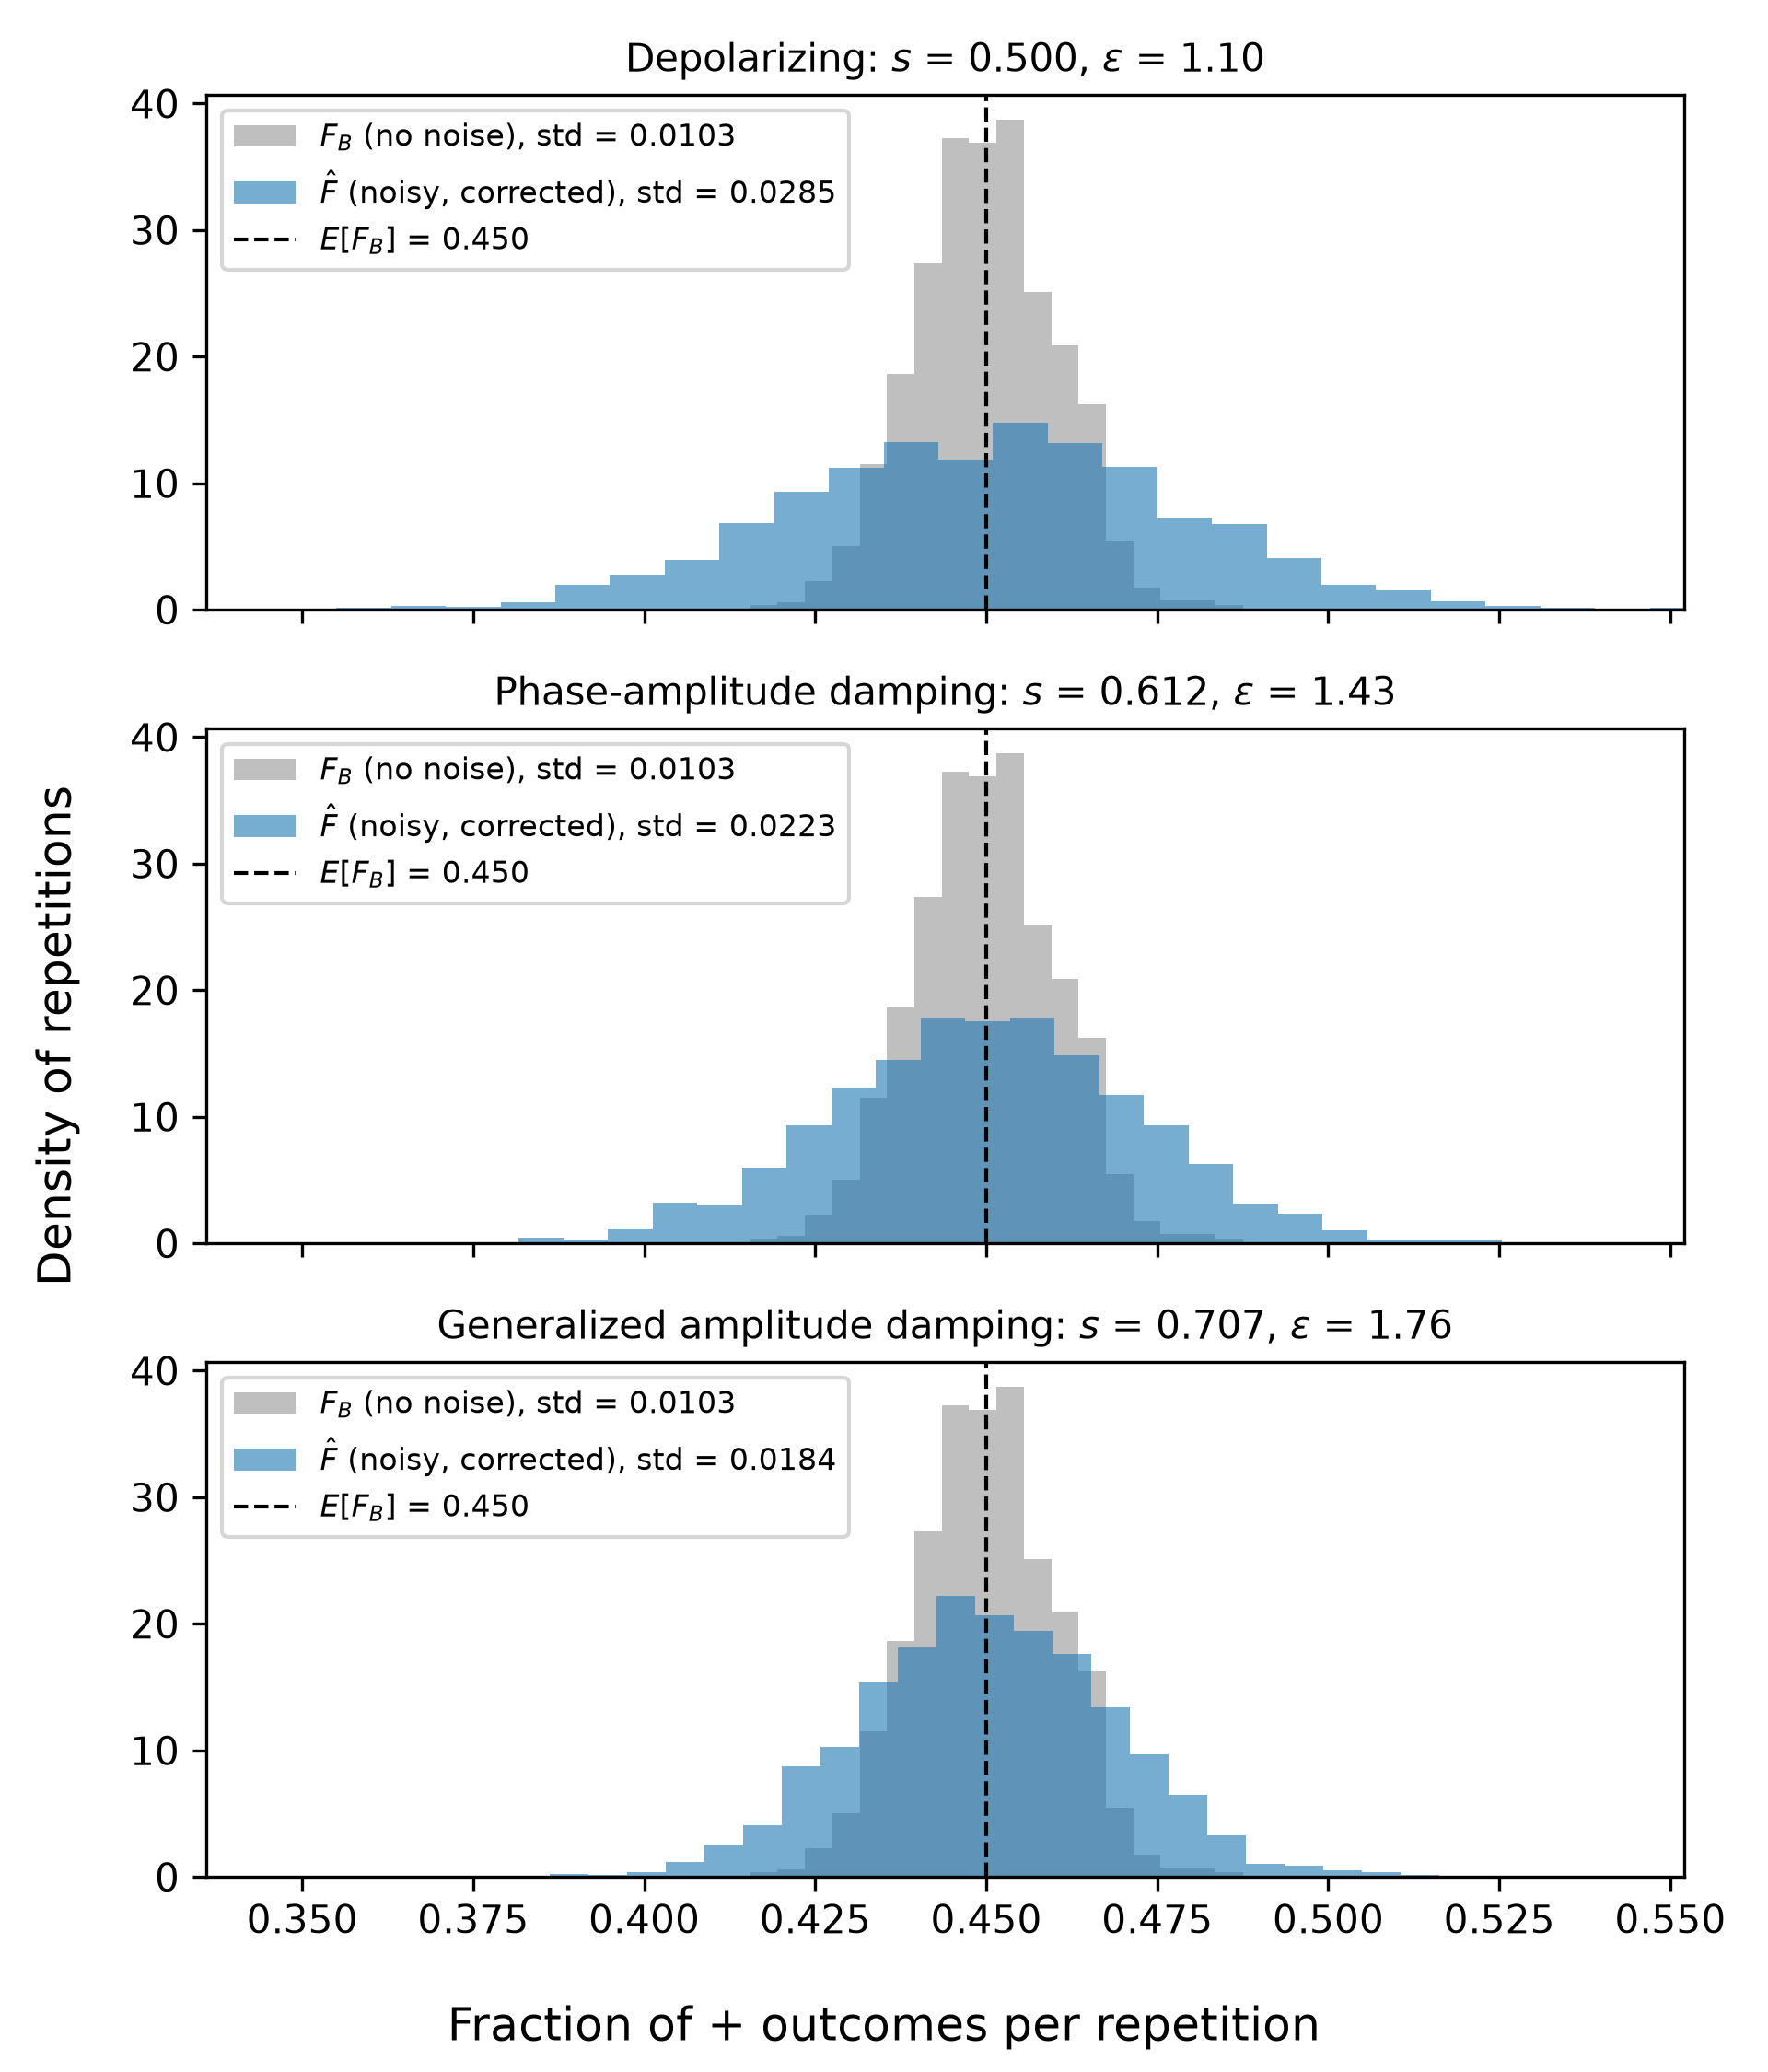
\includegraphics[width=\columnwidth]{histograma_collateral_mecanismos.png}
  \caption{Histograma de densidad de la fracción de personas cuyo estado medido fue $\ket{+}$, sin ruido ($F_B$) y después del ruido y la corrección ($\hat{F}$), para DEP, PAD y GAD (de arriba abajo)}
  \label{fig:measurement_histograms}
\end{figure}

Podemos observar que el valor medio de $F_C$ coincide con la teoría y que, después de la corrección $\hat{F}$, el valor medio vuelve al de $F_B$, pero la desviación estándar aumenta en todos los casos. Las desviaciones estándar simuladas están todas ligeramente por debajo de las teóricas, desde un $1.6\%$ (para $F_B$) hasta un $2.9\%$ (para $\hat{F}$ con PAD). Como $1/\sqrt{2R} \approx 1.6\%$ es el tamaño típico de este error (un error estándar), y cerca del $95\%$ de las ejecuciones caen dentro de dos errores estándar ($3.2\%$), estas diferencias son esperables. Además, todas se desvían en la misma dirección porque ambas ramas comparten los mismos números aleatorios, así que se trata de una sola fluctuación y no de cuatro independientes.

El cambio en la desviación estándar es el verdadero costo de la privacidad, que discutiremos con más detalle en la Sección~\ref{sec:discussion_and_conclusion}, pero directamente de los datos de la Tabla~\ref{tab:measurement_results} el lector puede observar que cada mecanismo da una desviación estándar $2.78$, $2.17$ y $1.80$ veces mayor que $\mathrm{std}(F_B)$, respectivamente. Esto se debe al denominador de la Ecuación~\eqref{eq:corrected_std}, que hace que la desviación estándar corregida sea inversamente proporcional al coeficiente de contracción, de modo que un $s$ más pequeño (más contracción) implica una desviación estándar mayor. Esto explica el compromiso fundamental de la privacidad diferencial: con un $s$ mayor (menos ruido), el $\epsilon$ será mayor porque las personas podrán distinguirse con más facilidad y, al mismo tiempo, el $\hat{F}$ corregido tendrá una distribución más precisa.

Por último, el lector habrá notado que los valores de $\epsilon_{meas}$ son los mismos que resultaron como $\epsilon_{exp}$ en el experimento del escenario local para \texttt{collateral}. Esto se debe en parte a la Proposición~\ref{prop:post_processing}, ya que la medición en sí es una operación cuántica y por lo tanto está acotada por el $\epsilon$ del mecanismo de ruido. Además, la variable \texttt{collateral} medida en $X$ distingue completamente el peor par sin ruido (carro y bienes raíces). Después del ruido, como muestra la Ecuación~\eqref{eq:epsilon_measurement_replaced}, el valor se alcanza para los estados que quedan a la mayor distancia de traza, $d=1$.


\section{Discusión y conclusiones}
\label{sec:discussion_and_conclusion}

La primera contribución de esta investigación fue un marco para codificar datos clásicos en estados cuánticos, que luego se usó en los experimentos propuestos para estudiar los efectos de la privacidad diferencial en simulaciones cuánticas.

En el experimento del escenario central encontramos qué tan holgado es $\epsilon_{theo}$ con respecto al resultado experimental $\epsilon_{exp}$. Como se muestra en la Ecuación~\eqref{eq:final_bound}, $\epsilon_{exp}$ es una cota inferior del verdadero presupuesto de privacidad, y por lo tanto el presupuesto real del conjunto de datos está en $[\epsilon_{exp}, \epsilon_{theo}]$. Como nuestra estimación nunca alcanzó esta cota superior, un curador que fije el presupuesto de privacidad en $\epsilon_{theo}$ tiene una garantía de privacidad, pero puede estar sacrificando utilidad a cambio de una privacidad que el conjunto de datos no necesita. El curador tampoco puede usar $\epsilon_{exp}$ en su lugar, ya que es solo una cota inferior.

En el escenario local, donde cada titular de los datos es responsable de agregar ruido a sus propios datos, el presupuesto de privacidad es mucho mayor (cerca de 1000 veces el del escenario central). A primera vista esto podría parecer un argumento directo para usar solo el escenario central al proteger datos; sin embargo, como se vio en la Sección~\ref{sec:measurement_release}, esto tiene un costo. Debido al teorema de no clonación, el analista necesita $N$ copias independientes para leer el estado central, así que el $\epsilon$ más pequeño se gasta $N$ veces, lo que da un presupuesto de privacidad total de $N\epsilon$ (Corolario~\ref{cor:composition}). Por otro lado, el presupuesto mayor del mecanismo local se gasta una sola vez, ya que cada persona mide su propio estado una sola vez. Para el único qubit de \texttt{collateral} con DEP y $N = 1000$ copias (el mismo número de resultados que recibe la publicación local, uno por persona), ninguno de los dos métodos es claramente mejor: en el escenario central $\epsilon_{tot} = 1000 \times 0.000608 = 0.608$, mientras que en el escenario local $\epsilon = 1.099$.

Por último, se podría intentar aplicar el ruido directamente sobre la matriz de densidad completa de 8 qubits, como lo permite el mecanismo DEP. Sin embargo, el $\epsilon$ resultante es entre 20 y 27 veces mayor que la suma de los presupuestos por qubit. Esto se debe a que en el Teorema~\ref{thm:epsilon_dep} $\epsilon$ crece con $D$: en la Definición~\ref{def:dep}, un $D$ más grande reparte el término de la identidad en más dimensiones, así que cada dirección recibe solo $p/D$ del ruido, mientras que $\rho$ se sigue comprimiendo solo por un factor de $(1-p)$. Como esta también es una publicación central, aplica el mismo razonamiento sobre la medición, y con $N = 1000$ copias el presupuesto total llega a $\epsilon_{tot} = 1000 \times 0.199849 = 199.849$, lo que hace que este método sea completamente inútil para proteger los datos.

Esta investigación también ofreció una forma de entender el verdadero costo de la privacidad. Como se vio en la Subsección~\ref{subsec:measurement_results}, después del ruido y la corrección la desviación estándar de $\hat{F}$ aumenta, lo que significa que los valores publicados quedan más dispersos alrededor de la media original. Ambos efectos provienen del mismo coeficiente de contracción $s$: un $s$ más pequeño reduce $\epsilon_{meas}$, de modo que un atacante tiene menos posibilidades de identificar a una sola persona, pero también amplía la desviación estándar, de modo que el analista obtiene una estimación menos precisa.

Esta investigación tiene dos limitaciones principales. Primero, los experimentos se realizaron en simuladores cuánticos, donde los canales de ruido se aplican de forma exacta mediante sus operadores de Kraus. En hardware real estas operaciones son más difíciles de llevar a cabo, ya que requieren qubits adicionales del entorno para producir la decoherencia y mediciones repetidas (\textit{shots}) para estimar los estados resultantes. Segundo, la codificación propuesta y los experimentos para medir el presupuesto de privacidad responden a elecciones específicas: el conjunto de datos German Credit y un único conjunto de parámetros de ruido (Tabla~\ref{tab:noise_params}).

En resumen, la investigación cumplió su objetivo, que era comparar y contrastar el presupuesto de privacidad teórico $\epsilon$ de distintos mecanismos de ruido cuántico con uno experimental en simulaciones de computación cuántica. Cada experimento produjo resultados que concuerdan con las expectativas fundamentadas en~\cite{zhou2017differential} y~\cite{dwork2014algorithmic}, entre muchos otros trabajos estudiados para llevar a buen término esta investigación. Como trabajo futuro proponemos implementar los mecanismos en hardware real, hacer barridos de parámetros, comparar con la QDP \textit{Lifted} de Song et al.~\cite{song2025hybrid}, y unir esta investigación con circuitos cuánticos variacionales para construir un flujo de aprendizaje automático cuántico privado.

\clearpage
\appendices

\renewcommand{\thelemma}{\Alph{section}.\arabic{lemma}}
\renewcommand{\theproposition}{\Alph{section}.\arabic{proposition}}

\section{Descripción de las variables seleccionadas}
\label{ap:selected_features}

La Tabla~\ref{tab:variables_descriptions} recopila el nombre, el tipo y la descripción de las variables seleccionadas para los experimentos cuánticos.

\begin{table*}[!t]
  \caption{Descripción de las variables seleccionadas.}
  \label{tab:variables_descriptions}
  \centering
  \begin{tabular}{llp{0.5\textwidth}}
    \toprule
    Nombre & Tipo & Descripción \\
    \midrule
    \texttt{status\_account}           & Categórica (ordinal)     & Estado de la cuenta corriente existente, en DM (marcos alemanes) \\
    \texttt{month\_duration}           & Numérica   & Duración del crédito en meses \\
    \texttt{credit\_amount}            & Numérica   & Monto del crédito \\
    \texttt{collateral}                & Categórica & Posible garantía del préstamo \\
    \texttt{purpose}                   & Categórica & Propósito del crédito \\
    \texttt{credit\_history}           & Categórica & Historial crediticio del solicitante \\
    \texttt{housing}                   & Categórica & Situación de vivienda actual (arriendo, propia o gratuita) \\
    \texttt{years\_employment}         & Categórica (ordinal)     & Tiempo en el empleo actual \\
    \texttt{status\_savings}           & Categórica (ordinal)     & Estado de la cuenta de ahorros, en DM (marcos alemanes) \\
    \texttt{other\_installment\_plans} & Categórica & Si el cliente tiene otros planes de pago a plazos \\
    \bottomrule
  \end{tabular}
\end{table*}

\section{Etiqueta asignada a cada categoría de las variables categóricas}
\label{ap:label_categorical}

La Tabla~\ref{tab:label_categorical} recopila las etiquetas asignadas a las categorías de cada variable usando la librería de Python scikit-learn.

\begin{table*}[!t]
  \caption{Asignación de la etiqueta de cada categoría de las variables categóricas}
  \label{tab:label_categorical}
  \centering
  \begin{tabular}{llc}
    \toprule
    Variable & Categoría & Etiqueta \\
    \midrule
    \multirow{4}{*}{\texttt{collateral}}
      & carro & 0 \\
      & ninguna & 1 \\
      & bienes raíces & 2 \\
      & acuerdo de ahorro/seguro de vida & 3 \\
    \midrule
    \multirow{10}{*}{\texttt{purpose}}
      & negocio & 0 \\
      & carro (nuevo) & 1 \\
      & carro (usado) & 2 \\
      & electrodomésticos & 3 \\
      & educación & 4 \\
      & muebles/equipos & 5 \\
      & otros & 6 \\
      & radio/televisión & 7 \\
      & reparaciones & 8 \\
      & recapacitación & 9 \\
    \midrule
    \multirow{5}{*}{\texttt{credit\_history}}
      & todos los créditos en este banco pagados a tiempo & 0 \\
      & cuenta crítica/otros créditos existentes (no en este banco) & 1 \\
      & retrasos en pagos en el pasado & 2 \\
      & créditos existentes pagados a tiempo hasta ahora & 3 \\
      & sin créditos tomados/todos los créditos pagados a tiempo & 4 \\
    \midrule
    \multirow{3}{*}{\texttt{housing}}
      & gratuita & 0 \\
      & propia & 1 \\
      & arriendo & 2 \\
    \midrule
    \multirow{3}{*}{\texttt{other\_installment\_plans}}
      & banco & 0 \\
      & ninguno & 1 \\
      & tiendas & 2 \\
    \bottomrule
  \end{tabular}
\end{table*}

\section{Correlación $\phi_{K}$ para todas las combinaciones de variables numéricas y ordinales}
\label{ap:phik_numerical_ordinal}

La Tabla~\ref{tab:phik_numerical_ordinal} muestra los resultados de correlación $\phi_{K}$ para todas las combinaciones de variables numéricas y ordinales, así como la peor correlación entre los dos pares.

\begin{table*}[htbp]
  \caption{Comparación de los pares de variables y métricas PhiK}
  \label{tab:phik_numerical_ordinal}
  \centering
  \setlength{\tabcolsep}{4pt}
  \begin{tabular}{@{}lllrrr@{}}
  \toprule
   & & & \multicolumn{3}{c}{$\phi_K$} \\
  \cmidrule(l){4-6}
  Sola & Primer par & Segundo par & Primer par & Segundo par & Peor \\
  \midrule
  \texttt{status\_account} & \texttt{status\_savings}, \texttt{month\_duration} & \texttt{years\_employment}, \texttt{credit\_amount} & 0.000 & 0.043 & 0.043 \\
  \texttt{credit\_amount} & \texttt{status\_account}, \texttt{years\_employment} & \texttt{status\_savings}, \texttt{month\_duration} & 0.088 & 0.000 & 0.088 \\
  \texttt{status\_savings} & \texttt{status\_account}, \texttt{month\_duration} & \texttt{years\_employment}, \texttt{credit\_amount} & 0.091 & 0.043 & 0.091 \\
  \texttt{status\_account} & \texttt{status\_savings}, \texttt{credit\_amount} & \texttt{years\_employment}, \texttt{month\_duration} & 0.092 & 0.065 & 0.092 \\
  \texttt{years\_employment} & \texttt{status\_account}, \texttt{month\_duration} & \texttt{status\_savings}, \texttt{credit\_amount} & 0.091 & 0.092 & 0.092 \\
  \texttt{month\_duration} & \texttt{status\_account}, \texttt{years\_employment} & \texttt{status\_savings}, \texttt{credit\_amount} & 0.088 & 0.092 & 0.092 \\
  \texttt{status\_savings} & \texttt{status\_account}, \texttt{credit\_amount} & \texttt{years\_employment}, \texttt{month\_duration} & 0.114 & 0.065 & 0.114 \\
  \texttt{years\_employment} & \texttt{status\_account}, \texttt{credit\_amount} & \texttt{status\_savings}, \texttt{month\_duration} & 0.114 & 0.000 & 0.114 \\
  \texttt{credit\_amount} & \texttt{status\_account}, \texttt{month\_duration} & \texttt{status\_savings}, \texttt{years\_employment} & 0.091 & 0.150 & 0.150 \\
  \texttt{month\_duration} & \texttt{status\_account}, \texttt{credit\_amount} & \texttt{status\_savings}, \texttt{years\_employment} & 0.114 & 0.150 & 0.150 \\
  \texttt{credit\_amount} & \texttt{status\_account}, \texttt{status\_savings} & \texttt{years\_employment}, \texttt{month\_duration} & 0.200 & 0.065 & 0.200 \\
  \texttt{month\_duration} & \texttt{status\_account}, \texttt{status\_savings} & \texttt{years\_employment}, \texttt{credit\_amount} & 0.200 & 0.043 & 0.200 \\
  \texttt{status\_account} & \texttt{status\_savings}, \texttt{years\_employment} & \texttt{credit\_amount}, \texttt{month\_duration} & 0.150 & 0.689 & 0.689 \\
  \texttt{status\_savings} & \texttt{status\_account}, \texttt{years\_employment} & \texttt{credit\_amount}, \texttt{month\_duration} & 0.088 & 0.689 & 0.689 \\
  \texttt{years\_employment} & \texttt{status\_account}, \texttt{status\_savings} & \texttt{credit\_amount}, \texttt{month\_duration} & 0.200 & 0.689 & 0.689 \\
  \bottomrule
  \end{tabular}
\end{table*}

\section{Ruido por qubit como mecanismo combinado}
\label{ap:composition_proof}

En este apéndice demostramos el Lema~\ref{lem:product_channel}, que se usa en la Sección~\ref{sec:finding_epsilon} para permitir la suma de los $\epsilon_{theo}^{k}$ y $\epsilon_{exp}^{k}$ de los $k$ qubits, mostrando que el producto tensorial de las salidas, $\bigotimes_i\mathcal{E}_i(\rho_i)$, es igual al producto tensorial de las operaciones aplicado al producto tensorial de los estados, $(\bigotimes_{i}\mathcal{E}_i)(\bigotimes_{i}\rho_i)$.

\begin{lemma}
  Sean $X_i$ y $U_i$ operadores lineales sobre un espacio vectorial $\mathcal{H}_i$, para $i = 1, \dots, k$. Entonces
  \[
    \Big(\bigotimes_{i=1}^{k} X_i\Big)\Big(\bigotimes_{i=1}^{k} U_i\Big) = \bigotimes_{i=1}^{k} X_i U_i.
  \]
  \label{lem:mixed_product}
\end{lemma}

\begin{IEEEproof}
  Dos operadores lineales son iguales si y solo si actúan de la misma forma sobre todo vector del espacio. Los vectores producto $e_1 \otimes \dots \otimes e_k$, con cada $e_i$ tomado de una base de $\mathcal{H}_i$, generan $\bigotimes_{i} \mathcal{H}_i$, y ambos lados son lineales, así que basta compararlos sobre estos vectores. Por la definición del producto tensorial de operadores, $(\bigotimes_i T_i)(\bigotimes_i v_i) = \bigotimes_i T_i v_i$~\cite[Ec.~(1.8)]{zwiebach2013tensor}.
  Por lo tanto
  \begin{align*}
    \Big(\bigotimes_{i} X_i\Big)\Big(\bigotimes_{i} U_i\Big)\Big(\bigotimes_{i} e_i\Big)
      &= \Big(\bigotimes_{i} X_i\Big)\Big(\bigotimes_{i} U_i e_i\Big) \\
      &= \bigotimes_{i} X_i U_i e_i \\
      &= \Big(\bigotimes_{i} X_i U_i\Big)\Big(\bigotimes_{i} e_i\Big),
  \end{align*}
  así que ambos operadores coinciden sobre todo vector producto, y por lo tanto sobre todo $\bigotimes_i \mathcal{H}_i$.
\end{IEEEproof}

\begin{proposition}
  Sea $A_i$ un operador lineal y $\rho_i$ un operador de densidad sobre $\mathcal{H}_i$, para $i = 1, \dots, k$. Entonces
  \begin{align*}
    \Big(\bigotimes_{i=1}^{k} A_i\Big)\Big(\bigotimes_{i=1}^{k} \rho_i\Big)&\Big(\bigotimes_{i=1}^{k} A_i\Big)^{\dagger} \\
      &= \bigotimes_{i=1}^{k} A_i \rho_i A_i^{\dagger}.
  \end{align*}
  \label{prop:product_operation}
\end{proposition}

\begin{IEEEproof}
  El adjunto de un producto tensorial es el producto tensorial de los adjuntos, $(\bigotimes_i A_i)^{\dagger} = \bigotimes_i A_i^{\dagger}$~\cite{Nielsen_Chuang_2010}.
  Aplicando dos veces el Lema~\ref{lem:mixed_product},
  \begin{align*}
    \Big(\bigotimes_{i} A_i\Big)\Big(\bigotimes_{i} \rho_i\Big)\Big(\bigotimes_{i} A_i^{\dagger}\Big)
      &= \Big(\bigotimes_{i} A_i\Big)\Big(\bigotimes_{i} \rho_i A_i^{\dagger}\Big) \\
      &= \bigotimes_{i} A_i \rho_i A_i^{\dagger}.
  \end{align*}
\end{IEEEproof}

\begin{IEEEproof}[Demostración del Lema~\ref{lem:product_channel}]
  La operación $\bigotimes_i \mathcal{E}_i$ tiene operadores de Kraus $E_{1,a_1} \otimes \dots \otimes E_{k,a_k}$, uno por cada elección de índices $a_1, \dots, a_k$. Aplicando la Proposición~\ref{prop:product_operation} a cada término, y luego la distributividad (bilinealidad) del producto tensorial sobre las sumas,
  \begin{align*}
    &\Big(\bigotimes_{i} \mathcal{E}_i\Big)\Big(\bigotimes_{i} \rho_i\Big) \\
    &\quad= \sum_{a_1, \dots, a_k} \Big(\bigotimes_{i} E_{i,a_i}\Big)\Big(\bigotimes_{i} \rho_i\Big)\Big(\bigotimes_{i} E_{i,a_i}\Big)^{\dagger} \\
    &\quad= \sum_{a_1, \dots, a_k} \bigotimes_{i} E_{i,a_i}\, \rho_i\, E_{i,a_i}^{\dagger} \\
    &\quad= \bigotimes_{i} \sum_{a_i} E_{i,a_i}\, \rho_i\, E_{i,a_i}^{\dagger}
       = \bigotimes_{i} \mathcal{E}_i(\rho_i).
  \end{align*}
\end{IEEEproof}

\clearpage
\raggedbottom

\bibliographystyle{IEEEtran}
\bibliography{references}


\EOD

\end{document}
